\documentclass[11pt]{article}

% The four macros of the header standard; tools/zenodo/publish_revision.py patches them when it reserves the DOI.
\newcommand{\doctype}{Preprint}
\newcommand{\docversion}{v1.00.000}
\newcommand{\docdate}{4 November 2026}
\newcommand{\versiondoi}{10.5281/zenodo.0}
\newcommand{\conceptdoi}{10.5281/zenodo.0}
\newcommand{\docidentity}{CAOS\_Contraste, the validation of the risk models of a bank}

% The packages and conventions every Contraste manuscript shares (CAOS_MANAGE conventions/manuscript-content-bar.md
% section 2). A document sets its class, the four header macros and \docidentity, then % The packages and conventions every Contraste manuscript shares (CAOS_MANAGE conventions/manuscript-content-bar.md
% section 2). A document sets its class, the four header macros and \docidentity, then % The packages and conventions every Contraste manuscript shares (CAOS_MANAGE conventions/manuscript-content-bar.md
% section 2). A document sets its class, the four header macros and \docidentity, then \input{../_shared/preamble}.
\usepackage[T1]{fontenc}
\usepackage[utf8]{inputenc}
\usepackage{lmodern}
\usepackage{microtype}
\usepackage[a4paper,margin=2.5cm]{geometry}
\usepackage{amsmath,amssymb,amsthm,mathtools,bm}
\usepackage{graphicx}
\usepackage{booktabs,longtable,tabularx,array,multirow}
\usepackage{siunitx}
\usepackage{algorithm}
\usepackage{algpseudocode}
\usepackage{caption,subcaption}
\usepackage{xcolor}
\usepackage[numbers,sort&compress]{natbib}
\usepackage[hidelinks]{hyperref}
\usepackage{cleveref}
\usepackage{orcidlink}

\sisetup{group-separator={,},group-minimum-digits=4,detect-all}
\graphicspath{{figures/}{../figures/}}
\captionsetup{font=small,labelfont=bf}
\setlength{\LTcapwidth}{\textwidth}

% Theorem environments for the Theory sections of the manuscripts.
\newtheorem{proposition}{Proposition}
\newtheorem{lemma}{Lemma}
\newtheorem{corollary}{Corollary}
\theoremstyle{definition}
\newtheorem{definition}{Definition}
\newtheorem{assumption}{Assumption}
\theoremstyle{remark}
\newtheorem{remark}{Remark}

% Notation shared by the documents (each defines it again in its notation table).
\newcommand{\E}{\mathbb{E}}
\newcommand{\Prob}{\mathbb{P}}
\newcommand{\Var}{\operatorname{Var}}
\newcommand{\Cov}{\operatorname{Cov}}
\newcommand{\VaR}{\operatorname{VaR}}
\newcommand{\ES}{\operatorname{ES}}
\newcommand{\PD}{\mathrm{PD}}
\newcommand{\LGD}{\mathrm{LGD}}
\newcommand{\EAD}{\mathrm{EAD}}
\newcommand{\ECL}{\mathrm{ECL}}
\newcommand{\indic}{\mathbf{1}}
\newcommand{\R}{\mathbb{R}}
\newcommand{\dd}{\,\mathrm{d}}

% The page-1 header block (CAOS_MANAGE conventions/manuscript-header-standard.md). The document defines \doctype,
% \docversion, \docdate, \versiondoi, \conceptdoi and \docidentity before this file; the publishing tool patches the four
% macros of the standard when it reserves the version DOI.
\newcommand{\docrepo}{github.com/fsantibanezleal/CAOS\_Contraste}
\newcommand{\headerblock}{%
\begin{center}
\fbox{\parbox{0.94\textwidth}{\small\raggedright
\textbf{\doctype} \quad$\cdot$\quad \docversion, \docdate \quad$\cdot$\quad Licence CC BY 4.0\\[2pt]
CAOS open-research programme \quad$\cdot$\quad \docidentity\\[2pt]
Version DOI \href{https://doi.org/\versiondoi}{\texttt{\versiondoi}} \quad$\cdot$\quad
concept DOI (always latest) \href{https://doi.org/\conceptdoi}{\texttt{\conceptdoi}}\\[2pt]
Not peer reviewed. Source code, data and computational records: \href{https://\docrepo}{\texttt{\docrepo}}
}}
\end{center}
\vspace{4pt}}
.
\usepackage[T1]{fontenc}
\usepackage[utf8]{inputenc}
\usepackage{lmodern}
\usepackage{microtype}
\usepackage[a4paper,margin=2.5cm]{geometry}
\usepackage{amsmath,amssymb,amsthm,mathtools,bm}
\usepackage{graphicx}
\usepackage{booktabs,longtable,tabularx,array,multirow}
\usepackage{siunitx}
\usepackage{algorithm}
\usepackage{algpseudocode}
\usepackage{caption,subcaption}
\usepackage{xcolor}
\usepackage[numbers,sort&compress]{natbib}
\usepackage[hidelinks]{hyperref}
\usepackage{cleveref}
\usepackage{orcidlink}

\sisetup{group-separator={,},group-minimum-digits=4,detect-all}
\graphicspath{{figures/}{../figures/}}
\captionsetup{font=small,labelfont=bf}
\setlength{\LTcapwidth}{\textwidth}

% Theorem environments for the Theory sections of the manuscripts.
\newtheorem{proposition}{Proposition}
\newtheorem{lemma}{Lemma}
\newtheorem{corollary}{Corollary}
\theoremstyle{definition}
\newtheorem{definition}{Definition}
\newtheorem{assumption}{Assumption}
\theoremstyle{remark}
\newtheorem{remark}{Remark}

% Notation shared by the documents (each defines it again in its notation table).
\newcommand{\E}{\mathbb{E}}
\newcommand{\Prob}{\mathbb{P}}
\newcommand{\Var}{\operatorname{Var}}
\newcommand{\Cov}{\operatorname{Cov}}
\newcommand{\VaR}{\operatorname{VaR}}
\newcommand{\ES}{\operatorname{ES}}
\newcommand{\PD}{\mathrm{PD}}
\newcommand{\LGD}{\mathrm{LGD}}
\newcommand{\EAD}{\mathrm{EAD}}
\newcommand{\ECL}{\mathrm{ECL}}
\newcommand{\indic}{\mathbf{1}}
\newcommand{\R}{\mathbb{R}}
\newcommand{\dd}{\,\mathrm{d}}

% The page-1 header block (CAOS_MANAGE conventions/manuscript-header-standard.md). The document defines \doctype,
% \docversion, \docdate, \versiondoi, \conceptdoi and \docidentity before this file; the publishing tool patches the four
% macros of the standard when it reserves the version DOI.
\newcommand{\docrepo}{github.com/fsantibanezleal/CAOS\_Contraste}
\newcommand{\headerblock}{%
\begin{center}
\fbox{\parbox{0.94\textwidth}{\small\raggedright
\textbf{\doctype} \quad$\cdot$\quad \docversion, \docdate \quad$\cdot$\quad Licence CC BY 4.0\\[2pt]
CAOS open-research programme \quad$\cdot$\quad \docidentity\\[2pt]
Version DOI \href{https://doi.org/\versiondoi}{\texttt{\versiondoi}} \quad$\cdot$\quad
concept DOI (always latest) \href{https://doi.org/\conceptdoi}{\texttt{\conceptdoi}}\\[2pt]
Not peer reviewed. Source code, data and computational records: \href{https://\docrepo}{\texttt{\docrepo}}
}}
\end{center}
\vspace{4pt}}
.
\usepackage[T1]{fontenc}
\usepackage[utf8]{inputenc}
\usepackage{lmodern}
\usepackage{microtype}
\usepackage[a4paper,margin=2.5cm]{geometry}
\usepackage{amsmath,amssymb,amsthm,mathtools,bm}
\usepackage{graphicx}
\usepackage{booktabs,longtable,tabularx,array,multirow}
\usepackage{siunitx}
\usepackage{algorithm}
\usepackage{algpseudocode}
\usepackage{caption,subcaption}
\usepackage{xcolor}
\usepackage[numbers,sort&compress]{natbib}
\usepackage[hidelinks]{hyperref}
\usepackage{cleveref}
\usepackage{orcidlink}

\sisetup{group-separator={,},group-minimum-digits=4,detect-all}
\graphicspath{{figures/}{../figures/}}
\captionsetup{font=small,labelfont=bf}
\setlength{\LTcapwidth}{\textwidth}

% Theorem environments for the Theory sections of the manuscripts.
\newtheorem{proposition}{Proposition}
\newtheorem{lemma}{Lemma}
\newtheorem{corollary}{Corollary}
\theoremstyle{definition}
\newtheorem{definition}{Definition}
\newtheorem{assumption}{Assumption}
\theoremstyle{remark}
\newtheorem{remark}{Remark}

% Notation shared by the documents (each defines it again in its notation table).
\newcommand{\E}{\mathbb{E}}
\newcommand{\Prob}{\mathbb{P}}
\newcommand{\Var}{\operatorname{Var}}
\newcommand{\Cov}{\operatorname{Cov}}
\newcommand{\VaR}{\operatorname{VaR}}
\newcommand{\ES}{\operatorname{ES}}
\newcommand{\PD}{\mathrm{PD}}
\newcommand{\LGD}{\mathrm{LGD}}
\newcommand{\EAD}{\mathrm{EAD}}
\newcommand{\ECL}{\mathrm{ECL}}
\newcommand{\indic}{\mathbf{1}}
\newcommand{\R}{\mathbb{R}}
\newcommand{\dd}{\,\mathrm{d}}

% The page-1 header block (CAOS_MANAGE conventions/manuscript-header-standard.md). The document defines \doctype,
% \docversion, \docdate, \versiondoi, \conceptdoi and \docidentity before this file; the publishing tool patches the four
% macros of the standard when it reserves the version DOI.
\newcommand{\docrepo}{github.com/fsantibanezleal/CAOS\_Contraste}
\newcommand{\headerblock}{%
\begin{center}
\fbox{\parbox{0.94\textwidth}{\small\raggedright
\textbf{\doctype} \quad$\cdot$\quad \docversion, \docdate \quad$\cdot$\quad Licence CC BY 4.0\\[2pt]
CAOS open-research programme \quad$\cdot$\quad \docidentity\\[2pt]
Version DOI \href{https://doi.org/\versiondoi}{\texttt{\versiondoi}} \quad$\cdot$\quad
concept DOI (always latest) \href{https://doi.org/\conceptdoi}{\texttt{\conceptdoi}}\\[2pt]
Not peer reviewed. Source code, data and computational records: \href{https://\docrepo}{\texttt{\docrepo}}
}}
\end{center}
\vspace{4pt}}

\makeatletter
\def\input@path{{sections/}}
% two algorithms: give the line anchors of each its own name, so that the hyperlinks do not collide
\def\theHALG@line{\thealgorithm.\arabic{ALG@line}}
\makeatother

% Notation of this manuscript, and the numbers of the text (generated by make_numbers.py from the committed documents).
\newcommand{\rej}{r}
\newcommand{\lev}{\alpha}
\newcommand{\nrep}{R}
\newcommand{\sev}{s}
\newcommand{\MCSE}{\widehat{\mathrm{SE}}}
\DeclareMathOperator{\Bin}{Bin}
\DeclareMathOperator{\Phin}{\Phi}
% Written by make_numbers.py from data/derived/C22 and experiments/results. Do not edit.

\newcommand{\nSims}{231}
\newcommand{\nReps}{551,000}
\newcommand{\nRates}{476}
\newcommand{\nExactRows}{47}
\newcommand{\nGens}{123}
\newcommand{\nFamilies}{8}
\newcommand{\nTests}{21}
\newcommand{\nPowerTests}{17}
\newcommand{\nTransition}{4}
\newcommand{\nNullReps}{4,000}
\newcommand{\nPowerReps}{2,000}
\newcommand{\fSimsNull}{28}
\newcommand{\fRepsNull}{128,000}
\newcommand{\fGensNull}{14}
\newcommand{\fSimsMiscal}{54}
\newcommand{\fRepsMiscal}{108,000}
\newcommand{\fGensMiscal}{24}
\newcommand{\fSimsCluster}{48}
\newcommand{\fRepsCluster}{96,000}
\newcommand{\fGensCluster}{24}
\newcommand{\fSimsDrift}{30}
\newcommand{\fRepsDrift}{60,000}
\newcommand{\fGensDrift}{12}
\newcommand{\fSimsDecay}{21}
\newcommand{\fRepsDecay}{60,000}
\newcommand{\fGensDecay}{17}
\newcommand{\fSimsLeak}{14}
\newcommand{\fRepsLeak}{27,000}
\newcommand{\fGensLeak}{8}
\newcommand{\fSimsBroken}{24}
\newcommand{\fRepsBroken}{48,000}
\newcommand{\fGensBroken}{18}
\newcommand{\fSimsConc}{12}
\newcommand{\fRepsConc}{24,000}
\newcommand{\fGensConc}{6}
\newcommand{\nExactCmp}{94}
\newcommand{\nExactNondeg}{63}
\newcommand{\nAgree}{94}
\newcommand{\zMaxAbs}{2.85}
\newcommand{\zSd}{1.20}
\newcommand{\zMean}{0.00}
\newcommand{\nHold}{12}
\newcommand{\nNotHold}{9}
\newcommand{\nHoldOneConfig}{10}
\newcommand{\nCompositeNull}{18}
\newcommand{\nHoldCellRule}{19}
\newcommand{\nNotHoldCellRule}{2}
\newcommand{\nHoldCellDef}{18}
\newcommand{\nNotHoldCellDef}{3}
\newcommand{\nHoldPoolRule}{14}
\newcommand{\nNotHoldPoolRule}{7}
\newcommand{\boundFivePool}{5.15}
\newcommand{\boundOnePool}{1.07}
\newcommand{\detIntFiveFour}{1.00}
\newcommand{\detIntOneFour}{0.47}
\newcommand{\flagIntFour}{5.2}
\newcommand{\detIntFiveTwoHundredK}{0.14}
\newcommand{\detIntOneTwoHundredK}{0.06}
\newcommand{\flagIntTwoHundredK}{5.0}
\newcommand{\intRateFiveFour}{5.70}
\newcommand{\intRateFiveTwoHundredK}{5.10}
\newcommand{\expFalseAboveExt}{1.3}
\newcommand{\expFalseAbove}{1.1}
\newcommand{\boundFive}{6.06}
\newcommand{\boundOne}{1.49}
\newcommand{\boundFiveBig}{5.48}
\newcommand{\jeffExactOne}{1.38}
\newcommand{\jeffExactFive}{4.79}
\newcommand{\jeffExcOne}{0.38}
\newcommand{\jeffSimOne}{1.12}
\newcommand{\jeffSimFive}{3.90}
\newcommand{\binExactFive}{4.79}
\newcommand{\binExactOne}{0.69}
\newcommand{\binSimFive}{4.55}
\newcommand{\normFive}{8.38}
\newcommand{\normOne}{4.05}
\newcommand{\normLoFive}{7.56}
\newcommand{\normHiFive}{9.27}
\newcommand{\migFive}{0.18}
\newcommand{\hhiFive}{0.0}
\newcommand{\momFive}{4.45}
\newcommand{\matFive}{3.70}
\newcommand{\ordFive}{6.05}
\newcommand{\timeFive}{4.72}
\newcommand{\ordLoFive}{5.35}
\newcommand{\ordHiFive}{6.83}
\newcommand{\ordOne}{1.47}
\newcommand{\ordLoOne}{1.15}
\newcommand{\ordHiOne}{1.90}
\newcommand{\ordTwentyK}{5.05}
\newcommand{\ordTwentyKLo}{4.76}
\newcommand{\ordTwentyKHi}{5.36}
\newcommand{\aucNullFive}{3.40}
\newcommand{\profileFive}{3.70}
\newcommand{\hlFive}{4.60}
\newcommand{\hlOne}{0.97}
\newcommand{\chiGradesFive}{5.30}
\newcommand{\markovBoundMargin}{0.01}
\newcommand{\hlFitted}{11.0}
\newcommand{\hlFittedOne}{3.4}
\newcommand{\hlDofTheory}{11.5}
\newcommand{\tlUpper}{6.35}
\newcommand{\tlUpperExact}{6.03}
\newcommand{\tlLowerExact}{3.79}
\newcommand{\chiThin}{5.67}
\newcommand{\chiThinOne}{1.73}
\newcommand{\aucDevOne}{11.6}
\newcommand{\aucDevOneExt}{5.3}
\newcommand{\aucDevTheory}{12.2}
\newcommand{\aucDevTheoryFour}{7.1}
\newcommand{\aucDevTheorySixteen}{5.5}
\newcommand{\psiHundred}{85.0}
\newcommand{\psiHundredTwentyFive}{22.9}
\newcommand{\psiHundredBench}{7.0}
\newcommand{\psiTheoryHundred}{83.4}
\newcommand{\psiTheoryHundredTF}{18.7}
\newcommand{\psiTheoryFourHundred}{1.8}
\newcommand{\binKOneTwoFive}{76.0}
\newcommand{\jeffKOneTwoFive}{79.8}
\newcommand{\hlKOneTwoFive}{64.9}
\newcommand{\spiKOneTwoFive}{94.6}
\newcommand{\chiKOneTwoFive}{66.1}
\newcommand{\normKOneTwoFive}{86.2}
\newcommand{\tlKOneTwoFive}{80.6}
\newcommand{\vasKOneTwoFive}{0.0}
\newcommand{\binKOneFive}{99.6}
\newcommand{\vasKOneFive}{0.0}
\newcommand{\vasKThree}{79.0}
\newcommand{\profKThree}{2.4}
\newcommand{\binKOneOne}{22.8}
\newcommand{\spiKOneOne}{41.2}
\newcommand{\hlKOneOne}{16.8}
\newcommand{\chiKOneOne}{16.0}
\newcommand{\vasKThreeExact}{78.8}
\newcommand{\binKOneTwoFiveExact}{74.9}
\newcommand{\binRhoTwo}{12.3}
\newcommand{\binRhoTwoExact}{13.2}
\newcommand{\binRhoFive}{17.5}
\newcommand{\binRhoFiveExact}{17.8}
\newcommand{\binRhoOneZero}{18.6}
\newcommand{\binRhoOneZeroExact}{19.7}
\newcommand{\chiRhoTwo}{46.8}
\newcommand{\chiRhoOneZero}{74.9}
\newcommand{\hlRhoTwo}{50.0}
\newcommand{\hlRhoTwoZero}{86.5}
\newcommand{\spiRhoFive}{34.5}
\newcommand{\normRhoFive}{7.4}
\newcommand{\normRhoTwoZero}{3.5}
\newcommand{\vasRhoOneZero}{4.7}
\newcommand{\vasRhoTwoZero}{5.9}
\newcommand{\tlRhoFive}{10.8}
\newcommand{\normRhoZero}{8.2}
\newcommand{\vasRhoTwoZeroExact}{7.1}
\newcommand{\psiBenchZeroTwo}{89.6}
\newcommand{\psiBenchZeroOne}{27.2}
\newcommand{\psiBandZeroOneAtZeroTwo}{2.8}
\newcommand{\psiBandZeroTwoFiveAtZeroTwo}{0.0}
\newcommand{\psiBandZeroOneAtZeroThree}{53.1}
\newcommand{\psiBandZeroTwoFiveAtZeroFive}{55.6}
\newcommand{\chiDriftZeroTwo}{88.5}
\newcommand{\ksDriftZeroTwo}{97.3}
\newcommand{\ksDriftZeroOne}{46.5}
\newcommand{\hlDriftZeroFive}{4.9}
\newcommand{\spiDriftZeroFive}{5.0}
\newcommand{\ecbDropZeroTwo}{25.4}
\newcommand{\ecbDropZeroFive}{81.5}
\newcommand{\ecbDropZeroEight}{99.1}
\newcommand{\delDropZeroFive}{71.6}
\newcommand{\delDropZeroTwo}{18.0}
\newcommand{\ecbDropAtPower}{0.049}
\newcommand{\delDropAtPower}{0.060}
\newcommand{\leakAucZeroTwoFive}{63.5}
\newcommand{\leakCsiZeroTwoFive}{6.0}
\newcommand{\leakCsiOne}{14.6}
\newcommand{\leakCsiTwo}{58.1}
\newcommand{\leakAucZeroFive}{98.9}
\newcommand{\migROneFivenFiveZeroZero}{7.9}
\newcommand{\migRTwonFiveZeroZero}{55.5}
\newcommand{\migRThreenFiveZeroZero}{99.7}
\newcommand{\migRTwonTwoZeroZeroZero}{100.0}
\newcommand{\migROneFivenTwoZeroZeroZero}{65.7}
\newcommand{\hhiPower}{0.0}
\newcommand{\chiCountZeroZeroFive}{94.8}
\newcommand{\chiCountZeroZeroTwo}{23.4}
\newcommand{\swapProfile}{95.2}
\newcommand{\swapChi}{93.7}
\newcommand{\hhiPeak}{1.09}
\newcommand{\hhiAllIn}{0.78}
\newcommand{\hhiAllInP}{0.22}
\newcommand{\zCrit}{1.645}
\newcommand{\nReach}{13}
\newcommand{\nNoReach}{4}
\newcommand{\sPsi}{0.185}
\newcommand{\sChiStab}{0.186}
\newcommand{\sKs}{0.166}
\newcommand{\sMig}{2.55}
\newcommand{\sBin}{1.29}
\newcommand{\sJeff}{1.25}
\newcommand{\sChi}{1.35}
\newcommand{\sHl}{1.36}
\newcommand{\sSpi}{1.21}
\newcommand{\sNorm}{1.23}
\newcommand{\sTl}{1.25}
\newcommand{\nMonoPairs}{220}
\newcommand{\nMonoViol}{0}
\newcommand{\wpAgree}{143}
\newcommand{\wpTotal}{144}
\newcommand{\wpRuns}{25,000}
\newcommand{\ynAgree}{50}
\newcommand{\ynTotal}{54}
\newcommand{\ynRuns}{10,000}
\newcommand{\ynMeanZ}{0.65}
\newcommand{\ynInterior}{52}
\newcommand{\demlerRuns}{1,000}
\newcommand{\demlerMeasured}{0.2}
\newcommand{\demlerPublished}{0.1}
\newcommand{\wpOffPub}{95.5}
\newcommand{\wpOffMeas}{94.4}
\newcommand{\ivWaldAll}{68}
\newcommand{\ivWaldNd}{56}
\newcommand{\ivWilsonAll}{87}
\newcommand{\ivWilsonNd}{57}
\newcommand{\ivACAll}{88}
\newcommand{\ivACNd}{57}
\newcommand{\ivCPAll}{88}
\newcommand{\ivCPNd}{57}
\newcommand{\ivJefAll}{87}
\newcommand{\ivJefNd}{56}
\newcommand{\covWaldThousandth}{90.6}
\newcommand{\covWaldOne}{94.4}
\newcommand{\covWaldFive}{94.9}
\newcommand{\covWilsonThousandth}{93.1}
\newcommand{\covWilsonOne}{95.4}
\newcommand{\covWilsonFive}{95.4}
\newcommand{\covACThousandth}{97.9}
\newcommand{\covACOne}{95.4}
\newcommand{\covACFive}{95.4}
\newcommand{\covCPThousandth}{96.0}
\newcommand{\covCPOne}{96.2}
\newcommand{\covCPFive}{95.4}
\newcommand{\covJefThousandth}{96.0}
\newcommand{\covJefOne}{94.4}
\newcommand{\covJefFive}{95.0}
\newcommand{\flagFive}{0.14}
\newcommand{\flagOne}{0.18}
\newcommand{\flagTest}{0.31}
\newcommand{\flagFamily}{6.4}
\newcommand{\flagThousand}{0.48}
\newcommand{\flagTwentyK}{0.25}
\newcommand{\detFiveThousand}{2.87}
\newcommand{\detOneThousand}{1.36}
\newcommand{\detFiveTwoK}{2.01}
\newcommand{\detOneTwoK}{0.94}
\newcommand{\detFiveFour}{1.39}
\newcommand{\detOneFour}{0.66}
\newcommand{\detFiveTwentyK}{0.61}
\newcommand{\detOneTwentyK}{0.28}
\newcommand{\detFiveTwoHundredK}{0.19}
\newcommand{\detOneTwoHundredK}{0.09}
\newcommand{\agFailOne}{0.1}
\newcommand{\agFailTwoPercent}{14.8}
\newcommand{\agFailFivePercent}{98.5}
\newcommand{\agFailTenPercent}{100.0}
\newcommand{\agSimFive}{99.0}
\newcommand{\agSimTen}{100}
\newcommand{\agSimNone}{0.0}
\newcommand{\agBlocks}{200}
\newcommand{\agMeanRateFive}{6.74}
\newcommand{\hhiWilsonHi}{0.10}
\newcommand{\jeffDetect}{28.1}
\newcommand{\jeffDetectInt}{64.2}
\newcommand{\nReproduced}{21}
\newcommand{\nReproTotal}{21}
\newcommand{\seedMinutes}{14}
\newcommand{\reproSeconds}{67}
\newcommand{\instrMinutes}{3.4}
\newcommand{\nBlocks}{50}
\newcommand{\nRepsPooled}{200,000}
\newcommand{\sdRatioMean}{1.00}
\newcommand{\sdRatioMin}{0.78}
\newcommand{\sdRatioMax}{1.22}
\newcommand{\nWithin}{10}
\newcommand{\nOver}{9}
\newcommand{\nNeither}{2}
\newcommand{\nVerdictAgree}{15}
\newcommand{\nVerdictDisagree}{6}
\newcommand{\nVerdictAgreeRule}{16}
\newcommand{\nVerdictDisagreeRule}{5}
\newcommand{\nMissedByCell}{6}
\newcommand{\nMissedByCellRule}{7}
\newcommand{\nPoolDefOnly}{2}
\newcommand{\smallExcMax}{0.29}
\newcommand{\smallExcMin}{0.05}
\newcommand{\nSmallOver}{7}
\newcommand{\pooledPsi}{5.29}
\newcommand{\pooledHl}{5.17}
\newcommand{\pooledSpi}{5.15}
\newcommand{\pooledOrd}{5.15}
\newcommand{\pooledChi}{5.15}
\newcommand{\pooledDel}{5.13}
\newcommand{\pooledCsi}{5.09}
\newcommand{\pooledHlOne}{1.26}
\newcommand{\pooledNorm}{7.99}
\newcommand{\pooledNormExc}{2.99}
\newcommand{\pooledNormLo}{7.87}
\newcommand{\pooledNormHi}{8.11}
\newcommand{\pooledDelLo}{5.034}
\newcommand{\pooledCsiLoOne}{1.003}
\newcommand{\pooledCsiOne}{1.05}
\newcommand{\pooledJeffOne}{1.38}
\newcommand{\pooledBinOne}{0.66}
\newcommand{\pooledMigFive}{0.11}
\newcommand{\pooledAucFive}{4.00}
\newcommand{\pooledProfFive}{4.05}
\newcommand{\pooledTlFive}{3.81}
\newcommand{\flWithinBoundThousand}{0.15}
\newcommand{\flWithinNaiveThousand}{22.7}
\newcommand{\flWithinIntThousand}{1.10}
\newcommand{\flOverIntThousand}{21.7}
\newcommand{\flOverBoundThousand}{13.0}
\newcommand{\flOverNaiveThousand}{77.6}
\newcommand{\flWithinBoundTwoK}{0.00}
\newcommand{\flWithinNaiveTwoK}{19.4}
\newcommand{\flWithinIntTwoK}{0.90}
\newcommand{\flOverIntTwoK}{27.4}
\newcommand{\flOverBoundTwoK}{13.7}
\newcommand{\flOverNaiveTwoK}{82.1}
\newcommand{\flWithinBoundFour}{0.00}
\newcommand{\flWithinNaiveFour}{14.0}
\newcommand{\flWithinIntFour}{1.60}
\newcommand{\flOverIntFour}{33.3}
\newcommand{\flOverBoundFour}{16.4}
\newcommand{\flOverNaiveFour}{87.8}
\newcommand{\flWithinBoundTwentyK}{0.00}
\newcommand{\flWithinNaiveTwentyK}{10.0}
\newcommand{\flWithinIntTwentyK}{0.00}
\newcommand{\flOverIntTwentyK}{62.2}
\newcommand{\flOverBoundTwentyK}{38.9}
\newcommand{\flOverNaiveTwentyK}{97.8}
\newcommand{\nStudies}{25}
\newcommand{\nExtTests}{21}
\newcommand{\nExtHold}{16}
\newcommand{\nExtNotHold}{5}
\newcommand{\nStudiesHold}{20}
\newcommand{\nStudiesNotHold}{5}
\newcommand{\nExtHoldRule}{19}
\newcommand{\nStudiesHoldRule}{23}
\newcommand{\extPowMin}{14}
\newcommand{\extPowMax}{100}
\newcommand{\extPowMed}{73.2}
\newcommand{\extAboveBar}{10}
\newcommand{\extBelowHalf}{4}
\newcommand{\lgdTimeOne}{1.47}
\newcommand{\mcConvFive}{5.88}
\newcommand{\duUncondFive}{5.78}
\newcommand{\chrIndFive}{5.7}
\newcommand{\chrIndOne}{1.52}
\newcommand{\chrCcFive}{6.9}
\newcommand{\aucCover}{94.0}
\newcommand{\aucCoverMcse}{0.4}
\newcommand{\aucSeRel}{-0.15}
\newcommand{\nConsFive}{7}
\newcommand{\nExtCons}{8}
\newcommand{\expFalseAboveFour}{1.1}
\newcommand{\flagUnion}{6.6}
\newcommand{\binLimitRhoFive}{39.6}
\newcommand{\binLimitRhoTen}{35.3}
\newcommand{\binNRhoTenThousand}{19.7}
\newcommand{\binNRhoTenTenK}{28.8}
\newcommand{\binNRhoTenHundredK}{34.3}
\newcommand{\hhiKMinSix}{22}
\newcommand{\hhiKMinThree}{9}
\newcommand{\nBinRecon}{26}
\newcommand{\binReconMax}{4.4\times10^{-10}}
\newcommand{\zBound}{3.090}
\newcommand{\zAgree}{3.29}


\title{Twelve of 21 credit-risk validation tests hold their size on 200,000 null repetitions: a measurement of size and power on generators of known truth}
\author{Felipe Santib\'a\~nez-Leal~\orcidlink{0000-0002-0150-3246}\\
\small CAOS open-research programme, Santiago, Chile\\
\small \texttt{fsantibanez@gmail.com}}
\date{\docdate}

\begin{document}
\maketitle
\headerblock

\begin{abstract}
Validation reports judge the risk of a model by statistical tests whose error rates the supervisory texts do not state.
We measure the size and power of each test on generators of known truth, under its null and under planted defects, with a Monte Carlo standard error and a Wilson interval for every rate and the exact probability where one exists.
A test holds its size unless its exact rejection probability or the Wilson interval of its rate lies above the level at 5\,\% or 1\,\%.
Of \nTests{} credit-risk tests, \nHold{} hold their size on \nRepsPooled{} null repetitions each and \nNotHold{} do not; the largest excesses are the Jeffreys test, with an exact size of \jeffExactOne\,\% at the 1\,\% level, and the normal test over five years, which rejects \pooledNorm\,\% of correct models at 5\,\% (Wilson interval \pooledNormLo\ to \pooledNormHi\,\%). For \nHoldOneConfig{} of the \nHold{} the null is composite and the size is measured at one configuration.
Cells of \nNullReps{} repetitions resolve \detIntFiveFour{} point and show \nHoldCellDef{} holding, so the count depends on them.
Tests that assume independent defaults reject a correct PD in \binRhoOneZeroExact\,\% of samples at an asset correlation of 10\,\%, the 0.10 rule of the stability index alarms in \psiHundred\,\% of unchanged samples of 100, and the European Central Bank's concentration test cannot reject at 5\,\% with ten grades at an initial coefficient of variation of 0.6.
Of \nPowerTests{} power curves, \nReach{} reach 80\,\% on their ladder; a planted ladder is not a real bank.

\end{abstract}

\section{Introduction}
\label{sec:introduction}

A bank that uses a model to price credit, set provisions or hold capital must show, on a regular schedule, that the model still does what it was built to do.
The evidence is a battery of statistical tests: a test of whether the default rates that occurred are consistent with the probabilities of default the model assigned, a test of whether the model still ranks defaulters above survivors, an index of whether the population it scores has moved, a test of whether the rating migrations still obey the monotonicity the rating scale promises.
Each test returns a p-value, the p-value is read against a level, and the result is a light, green, amber or red, that goes into a report which a committee reads and a supervisor may inspect.
The 2011 supervisory guidance on model risk management, since replaced in the United States but still the reference text of the practice that followed, lists outcomes analysis, including back-testing, among the three core elements of validation \citep{fed2011sr117}, and the European Central Bank prescribes the tests that an institution reports for its internal ratings-based models \citep{ecb2019instructions}.

A decision rule that is read every quarter has two error rates, and a reader who acts on its light needs both.
The size of a test is the probability that it rejects a model that satisfies the null hypothesis; the power is the probability that it rejects a model that has a given defect \citep{neymanpearson1933}.
The texts that define the tests state neither.
The instructions of the European Central Bank define the tests and set no thresholds for pass or fail \citep{ecb2019instructions}; the study of validation methods of the Basel Committee concludes that no really powerful tests of adequate calibration are currently available \citep{bcbswp14}; and the population stability index is applied with bands whose type~I and type~II errors were first derived only recently \citep{yurdakul2020}.
Published size and power studies exist for a few tests, one for the normal test and the traffic-lights test of the Basel Committee, one for the stability index, one for the comparison of areas under the ROC curve on nested models \citep{bcbswp14,yurdakul2020,demler2012}.
None of them covers a battery under one protocol, and in the documentation of the validation toolkits read for this study the tests are listed with thresholds and traffic lights and no measured size or power is recorded; that statement is limited to the documentation that was read.

The gap matters because the answer is not obvious from the form of a test.
A test can be exact under its assumptions and badly sized when one assumption fails, and the assumptions of the validation tests fail in the ways that real portfolios fail: defaults are correlated, the reference value of a statistic is itself an estimate, a rule of thumb has a fixed threshold that ignores the sample size, a Bayesian interval is used as a frequentist test on a discrete count.
A test can also be valid and blind: it holds its size and cannot see the defect that a validator expects it to see.
With real outcomes neither property can be measured, because the truth about the model is unknown.
On a generator whose truth is known, both can.

\paragraph{The proposed measurement.}
We measure the size and the power of each test of a validation battery on generators of known truth.
A generator is a frozen configuration with an exact truth; the test is called exactly as a validator calls it; the null is the generator at the boundary of the test's null hypothesis with every assumption met; a defect is a departure planted in the generator at six severities along a ladder.
Every rejection rate carries its Monte Carlo standard error and its Wilson interval; where the rejection probability can be computed without simulation, the exact value is placed beside the simulated rate, which checks the generator, the harness and the test together; a test is said to hold its size when its rate does not exceed the level by more than the Monte Carlo error allows, or when its exact probability does not exceed the level.
Each repetition draws from an independent random stream spawned from one seed, so that any repetition reruns alone.
The design follows the structure that \citet{morris2019} recommend for simulation studies, and every rate carries the Monte Carlo standard error that their review found missing from most of the published studies it examined.

\paragraph{Contributions.}
\begin{enumerate}
\item A measurement protocol for the size and power of validation tests, with its estimator, its error, its exact checks and its decision rules stated as equations and as two algorithms (\cref{sec:proposed-method}).
\item Propositions on the error of the measurement itself: the probability that the size judgement flags a correct test, the smallest excess that a given number of repetitions can see, and the monotonicity that exact power curves must have, together with derivations of why four families of tests fail their level (\cref{sec:theory}).
\item The measured size of \nTests{} tests and the measured power of \nPowerTests{} of them, from \nSims{} simulations and \nReps{} seeded repetitions in \nFamilies{} families, with \nRates{} rates, every one with its standard error and its Wilson interval (\cref{sec:results}).
\item Evidence that the instrument is sound: \nExactRows{} rows carry an exact probability and all \nAgree{} comparisons agree within 3.29 standard errors; the three published simulation studies that can be rerun are rerun; every committed count reproduces exactly from its seed; fifty independent replications show how far the judgement of one cell can be trusted (\cref{sec:results,sec:ablation}).
\item An extension to \nExtTests{} further tests of counterparty, provisioning, loss-given-default, market, portfolio, fairness and machine-learning families at one stated alternative each (\cref{sec:extension}).
\end{enumerate}

\paragraph{Main results.}
Of the \nTests{} tests, \nHold{} hold their size at the 5\,\% and 1\,\% levels.
The two that do not are the Jeffreys test of the default probability, whose exact size is \jeffExactOne\,\% at the 1\,\% level, and the normal test over five years, which rejects \normFive\,\% of correct models at the 5\,\% level.
A cell of \nNullReps{} repetitions cannot see an excess smaller than about \detFiveFour{} points at the 5\,\% level, and a rerun of each test in \nBlocks{} independent blocks, \nRepsPooled{} repetitions in all, shows that \nSmallOver{} further tests exceed their level by \smallExcMin{} to \smallExcMax{} points.
The assumptions behind the lights matter more than these excesses.
A test that assumes independent defaults rejects a correct PD in \binRhoOneZeroExact\,\% of samples when the asset correlation of the defaults is 10\,\% (exact value, portfolio of 1,000 obligors), the 0.10 rule of the population stability index raises a false alarm in \psiHundred\,\% of samples of 100 in which nothing changed, and the concentration test of the European Central Bank cannot reject at 5\,\% with ten grades and an initial coefficient of variation of 0.6, because its statistic never exceeds \hhiPeak.
On power, \nReach{} of the \nPowerTests{} tests reach 80\,\% on the ladder of the defect planted for them, and the default-profile test, the Vasicek-corrected binomial test, the characteristic stability index and the concentration test do not.

\paragraph{Structure.}
\Cref{sec:related-work} places the measurement among the published tests, simulation methodology and interval estimators.
\Cref{sec:problem} defines size, power and the estimands.
\Cref{sec:proposed-method} gives the measurement in full, and \cref{sec:theory} its theory.
\Cref{sec:experimental-design} states the predictions, the data and the experiments; \cref{sec:results} reports them and \cref{sec:ablation} removes one component of the protocol at a time.
\Cref{sec:discussion,sec:limitations} interpret the results and bound them, \cref{sec:reproducibility} gives the commands that rebuild every number, and \cref{sec:conclusions} concludes.

\section{Related work}
\label{sec:related-work}

\subsection{Supervisory texts and the missing error rates}
\label{sec:rw-supervisory}

The 2011 guidance on model risk management of the United States supervisors names outcomes analysis, which includes back-testing, among the three core elements of validation, beside the evaluation of conceptual soundness and ongoing monitoring \citep{fed2011sr117}.
The reporting instructions of the European Central Bank for internal ratings-based models define the statistics a bank reports for calibration, discrimination, rating stability and concentration, and attach to them no threshold for pass or fail \citep{ecb2019instructions}.
The study of validation methods of the Basel Committee on Banking Supervision reviews the calibration tests of its time, simulates the normal test and the traffic-lights test, and concludes that no really powerful tests of adequate calibration are currently available \citep{bcbswp14}; the newsletter on low-default portfolios addresses the case in which a portfolio produces too few defaults for any of these tests to be informative \citep{bcbs2005lowdefault}.
These texts specify what to compute.
They do not give, for the statistics they prescribe, the rate at which a correct model is flagged or a defective one is missed, and the validator is left to read a p-value without the error rate that would say what the p-value is worth.

\subsection{Tests of the default probability}
\label{sec:rw-calibration}

The tests of calibration used in practice descend from a few constructions.
The binomial test and its extension to correlated defaults, which rests on the single-factor model of the capital rules \citep{gordy2003}, treat the number of defaults of a portfolio as a binomial count, or as a binomial mixture over one systematic factor; the traffic-lights approach colours each year's standardised default rate and rejects on the profile of colours; the normal test aggregates the differences between forecast and observed rates over several years \citep{bcbswp14}.
A Bayesian reading of the same count, with the Jeffreys prior \citep{jeffreys1946}, gives the posterior probability that the true default probability lies below the one applied, which the European Central Bank prescribes for its reporting \citep{ecb2019instructions}.
The chi-square statistic of Pearson \citep{pearson1900} over grades and the default-profile test, which compares the distribution of defaults over grades with the one the curve implies \citep{tasche2013}, test the shape of the calibration; the review of \citet{tasche2008} treats the validation of internal rating systems and of probability-of-default estimates, and the volume edited by \citet{engelmann2011} places these tests among the validation of the Basel risk parameters.
At obligor level the Hosmer--Lemeshow statistic groups obligors by predicted probability \citep{hosmer1980}, its power depends on the sample size and on the grouping \citep{hosmer1997,paul2013}, and the Spiegelhalter statistic standardises the Brier score without any binning \citep{spiegelhalter1986,brier1950}.
Of these, the simulation of \citet{bcbswp14} measures the size and power of two tests on eight scenarios; no source known to us measures the other tests, with the same protocol and the same generators, beside them.

\subsection{Discrimination and stability}
\label{sec:rw-discrimination}

The area under the ROC curve is the probability that a defaulter is ranked above a survivor \citep{hanley1982}; its standard error follows from the placement values of the defaulters and of the survivors, and the comparison of two areas on the same obligors by the covariance of their placements is the test of \citet{delong1988}.
\citet{demler2012} show by simulation that the DeLong test, applied to nested models fitted on the comparison sample, rejects a true null far below its level, so that the test is conservative and loses power for small and moderate effects in that design; their single published rate is one of the studies the measurement reruns.
A coherent alternative to the area as a measure of classifier performance has been proposed \citep{hand2009}; it does not change what the tests of the area measure, but it bears on what a validator should conclude from them.
For population stability, the index used in credit scoring is a symmetrised divergence between two binned distributions, applied with the bands of 0.10 and 0.25; \citet{yurdakul2020} derive its asymptotic distribution, which depends on the sizes of both samples and on the bins, observe that the bands are used without reference to type~I or type~II error rates, and report a simulation that the measurement reruns cell by cell.
The two-sample Kolmogorov--Smirnov test \citep{smirnov1948} and the chi-square test of homogeneity \citep{pearson1900} are the stability tests whose reference distributions are known in large samples.

\subsection{Rating transitions and multiplicity}
\label{sec:rw-transitions}

The tests of whether a rating process is a time-homogeneous Markov chain of first order are those of \citet{andersongoodman1957}, applied to the transition counts of a rating system.
The reporting instructions of the European Central Bank add a test per cell of a migration matrix that the frequency of a transition should not increase with the distance from the diagonal \citep{ecb2019instructions}; a matrix of seven grades has 42 such cells, so the control of multiplicity decides the size and the power of the family.
The sequentially rejective procedure of \citet{holm1979} controls the family-wise error rate without assuming independence, and the product bound of \citet{sidak1967} gives the probability that at least one of $m$ independent tests of level $\gamma$ rejects.
Both ideas enter the measurement: the first inside one test, the second in the judgement of a battery. Multiplicity matters more for the power of the migration test than for its size: with 42 cells the adjusted threshold of any one cell lies far below the nominal level, so the family-wise p-value of a single planted cell is conservative, which is the case that the measurement quantifies. The battery also holds a test of whether the transition counts of a year match a reference matrix and a test of downward rating momentum, for which only the size is measured.

\subsection{Back-tests of market and portfolio risk}
\label{sec:rw-backtests}

The proportion-of-failures test of \citet{kupiec1995}, the independence and conditional-coverage tests of \citet{christoffersen1998}, and the tests of the whole forecast density of \citet{berkowitz2001} are the tests on which the back-testing of value-at-risk rests, and \citet{nolde2017} distinguish such traditional back-tests, which assess whether a set of risk-measure forecasts is correct, from comparative back-tests, which compare two estimation procedures.
The measurement covers the tests of this family that the engine registers as a second part (\cref{sec:extension}), each against one stated alternative, because their natural ladders are not shared across tests. The proportion-of-failures test is a likelihood-ratio test of the number of exceedances of a value-at-risk forecast against its nominal rate; the independence test of \citet{christoffersen1998} is a likelihood-ratio test of a first-order Markov chain for the sequence of exceedances, and the conditional-coverage test combines the two. The proportion-of-failures and independence tests rest on asymptotic chi-square distributions, and the documentation of the engine reports that the asymptotic Kupiec test is not of nominal size at 250 days and a 1\,\% level, so the size of these tests in short series is in question.

\subsection{Simulation studies and error-rate reporting}
\label{sec:rw-simulation}

Size and power are the two error probabilities of a test in the sense of \citet{neymanpearson1933}.
Their estimation by simulation is the subject of a methodological literature: \citet{burton2006} set out how a simulation study in medical statistics should be designed, \citet{morris2019} organise it as aims, data-generating mechanisms, estimands, methods and performance measures, tabulate the Monte Carlo standard error of each performance measure, and report that most of the studies of a volume of a leading journal did not give one, and \citet{siepe2024} propose a template for planning, preregistering and reporting such studies.
The measurement follows that structure, and it adds what a validation battery needs: an exact probability beside the simulated rate where one exists, a decision rule for the size that is one-sided and accounts for the Monte Carlo error, and a statement of the smallest excess that the number of repetitions can resolve. The three works agree that a simulation study states its data-generating mechanisms and its performance measures before it reports results and that it reports the Monte Carlo error of each estimate; they do not address a battery of tests under one protocol, the exact probability beside the simulated rate, or the resolution of a size judgement.

\subsection{Intervals for a rate}
\label{sec:rw-intervals}

A rejection rate is a binomial proportion, and the choice of its interval matters most where the rates sit: at 1\,\% and below.
Five intervals are in common use: the score interval of \citet{wilson1927}, the exact interval of \citet{clopper1934}, the adjusted interval of \citet{agresti1998}, the equal-tailed Jeffreys interval, and the interval based on the normal approximation.
\citet{newcombe1998} compared seven methods for the interval of a single proportion, and \citet{brown2001} recommend the Wilson and the Jeffreys intervals for small samples and the interval of Agresti and Coull for larger ones, and find that the interval based on the normal approximation has poor coverage even for large samples when the proportion is small.
The measurement reports the Wilson interval and tests that choice against the others in \cref{sec:ablation}. A rejection rate near zero is where the choice matters: a rate of 0.1\,\% in 4,000 repetitions is four rejections, an interval built on the estimated variance is symmetric around a rate whose sampling distribution is not, and a rate of zero rejections gives it a zero width.

\subsection{Where the measurement stands}
\label{sec:rw-position}

The published work gives the tests, the supervisory texts prescribe them, and a few studies measure the error rates of a few of them.
The measurement proposed here treats a battery as one object: the same protocol, the same estimator and the same error for every test, an exact value as a check of the instrument where the test admits one, the published studies rerun inside it as a validation of the protocol, and a statement of the resolution of the result.
It does not propose a new test, and it does not claim that the generators represent any bank. Against the study of the Basel Committee, which simulates two tests on eight scenarios, and the stability study, which simulates one index on six pairs of sample sizes, the measurement differs in coverage, in protocol and in what it reports about itself: 21 tests of five families under one protocol, an exact check of the instrument, and the resolution of each judgement.

\section{Problem formulation}
\label{sec:problem}

\subsection{A validation test as a decision rule}
\label{sec:pf-rule}

A validation test $T$ takes the data $Y$ of a validation sample, such as the default counts of a portfolio, the scores and outcomes of its obligors, or two samples of a model input, and returns a p-value $p_T(Y)\in[0,1]$, or no p-value when its statistic is undefined, for example when a variance is zero.
At a level $\lev$ the test rejects when the p-value falls below it, $p_T(Y)<\lev$; the engine that is measured colours a result amber below 5\,\% and red below 1\,\%, and the two levels of the measurement are these, $\lev\in\{0.05,0.01\}$.
A result without a p-value is never a rejection and is counted separately.
Let $G_\theta$ be a generator of validation samples with parameter $\theta$ and exactly known truth, and let the \emph{rejection probability} of the test at level $\lev$ be
\begin{equation}
\rej_T(\theta,\lev)\;=\;\Prob_\theta\big(p_T(Y)<\lev\big),\qquad Y\sim G_\theta .
\label{eq:rejection}
\end{equation}
Every defect of a model is a departure of $\theta$ from the set $\Theta_0(T)$ of the parameters for which the null hypothesis of $T$ holds. Some tests are one-sided, as the binomial test whose alternative is a probability of default above the one applied, and some are two-sided, as the DeLong comparison of two areas; the rejection rule is the same for both, and only the null set differs.

\subsection{Size, power and the estimands}
\label{sec:pf-estimands}

The size of the test is the largest rejection probability over the null set, and its power at a parameter outside it is the rejection probability there:
\begin{equation}
\mathrm{size}_T(\lev)\;=\;\sup_{\theta\in\Theta_0(T)}\rej_T(\theta,\lev),\qquad
\mathrm{power}_T(\theta,\lev)\;=\;\rej_T(\theta,\lev),\quad \theta\notin\Theta_0(T).
\label{eq:size-power}
\end{equation}
For the three tests whose rejection region is a single default count, the null is one-sided in the probability of default, along which the rejection probability does not decrease (\cref{prop:monotone}); at the correlation that the test assumes, the supremum is then attained at the boundary of the null, the generator $G_{\theta_b}$ in which the null holds with equality and every assumption of the test is met, and the size is $\rej_T(\theta_b,\lev)$.
For the other eighteen tests the null set contains nuisance parameters: any common distribution of two samples (the stability indexes and the tests of homogeneity), any vector of probabilities of default (the chi-square, Hosmer--Lemeshow and Spiegelhalter tests), any path of yearly probabilities (the normal and traffic-lights tests), any correlation between two scores (DeLong), any common value of the area, the concentration or the migration frequency that is compared (the discrimination, concentration and migration tests), any transition chain (the four tests of transitions).
For these the measurement does not take the supremum: it measures the rejection probability $\rej_T(\theta_b,\lev)$ at one null configuration, which is a lower bound on the size, and the statement that a test holds its size at that configuration says nothing of the other configurations of the null (the Jeffreys case in \cref{sec:li-external} shows how much a rate can move with the configuration).
\emph{Evidence} about $\rej_T(\theta_b,\lev)$ is its exact value where the test has one, or a rate $\hat\rej$ in $\nrep$ repetitions with its Wilson interval $[\ell,u]$ of \eqref{eq:se-wilson}, and the evidence \emph{shows an excess} at the level $\lev$ when the exact value is above $\lev$ or when $\ell>\lev$.
\begin{definition}[Holding a size]
\label{def:holds}
A test \emph{holds its size on a body of evidence} when the evidence shows no excess at either level, $\lev\in\{0.05,0.01\}$. It is \emph{conservative} at a level when the exact value, or the whole interval, lies below the level, and it \emph{does not hold its size} when the evidence shows an excess at one of the levels.
\end{definition}
Every count of tests that hold their size in this paper, in the title, the abstract, the results and the conclusions, applies \cref{def:holds} and names its evidence. The count is a statement about the evidence and not only about the test: a test that holds its size on a cell of 4,000 repetitions may exceed its level by less than the resolution of the cell (\cref{prop:resolution}), and a test shown above its level by 200,000 repetitions may exceed it by a small fraction of a point. The one-sided bound of \cref{sec:pm-judgement}, which the pipeline applies to every cell and which tolerates a larger excess, is reported beside the definition under the name of the screen, never instead of it.

A defect is a one-parameter family $\theta(\sev)$ of generators, with a severity $\sev$ on a ladder of six values, and the power curve of the test against it is $\sev\mapsto\rej_T(\theta(\sev),\lev)$.
The summary of a curve that the measurement reports is the severity at which the power first reaches 80\,\%,
\begin{equation}
\sev_{0.8}(T)\;=\;\inf\{\sev:\ \rej_T(\theta(\sev),0.05)\ge 0.8\},
\label{eq:s80}
\end{equation}
which is a property of the test and the ladder together and carries the unit of the ladder.
The estimands are therefore the size at 5\,\% and at 1\,\% of each test at the boundary of its null, its power at each point of the ladder of each defect that it targets, and $\sev_{0.8}$; for the three tests whose rejection region is a single default count, they are also computable exactly.

\subsection{The tests that are measured}
\label{sec:pf-tests}

The battery is the 21 tests of the five credit families of the engine that return a p-value: nine tests of the calibration of the default probability, two of discrimination, four of population and characteristic stability, two of the rating system, and four of rating transitions.
\Cref{tab:tests} lists each with its statistic and its null hypothesis, as the engine documents them.
The four transition tests have a size in the measurement and no power, because no ladder of a defect of the transition process is planted for them, and the measurement does not claim a power for them. The 21 tests of the other seven families of the engine are measured separately (\cref{sec:extension}), each at the null of a named study and at one stated alternative.

\begin{table}[htbp]
\centering
\footnotesize
\caption{The 21 tests of the credit families that are measured: the statistic each computes and the null hypothesis it tests, as documented by the engine; D is the number of defaults, N the number of obligors, and a grade is a rating class.}
\label{tab:tests}
\fitwidth{\begin{tabular}{p{3.0cm}p{5.0cm}p{6.4cm}}
\toprule
Test & Statistic and reference distribution & Null hypothesis \\
\midrule
Binomial & upper tail of $\Bin(N,\mathrm{PD})$ at $D$ & true PD not above the PD applied, defaults independent \\
Jeffreys & posterior $\mathrm{Beta}(D+\tfrac12,N-D+\tfrac12)$ at the PD applied & PD applied not below the true PD \\
Vasicek-corrected binomial & binomial mixture over one systematic factor, assumed asset correlation & true PD not above the PD applied at the assumed correlation \\
Chi-square over grades & $\sum_i (n_ip_i-d_i)^2/(n_ip_i(1-p_i))$, $\chi^2$ with one degree of freedom per grade & every grade PD is the true one, defaults independent \\
Default profile & Pearson statistic of the defaults over grades given their number, Monte Carlo p-value & defaults fall on the grades as the PD curve implies (the shape, not the level) \\
Hosmer--Lemeshow & groups by predicted PD, $\chi^2$ with $G$ degrees of freedom for given PDs & predicted equals true PD in every group \\
Spiegelhalter & standardised Brier score, normal tail & the forecast equals the true PD of every obligor \\
Normal, five years & $\sum_t(d_t-\mathrm{PD}_t)/(\sqrt T\hat\sigma)$, normal tail & no year's true PD exceeds its forecast, years independent \\
Traffic lights & multinomial profile of the colours of the yearly standardised default rates, exact enumeration & as the normal test, with the colour probabilities of the rule \\
AUC against development & $(\mathrm{AUC}_\mathrm{dev}-\mathrm{AUC}_\mathrm{cur})/s$, normal tail, development AUC taken as known & AUC at development smaller than in the observation period \\
DeLong & difference of two AUCs on one sample over its covariance-based standard error, two-sided & the two AUCs are equal \\
Population stability index & PSI against $(1/n+1/m)\chi^2_{1-\lev,B-1}$ (chi-square benchmark) & the binned distributions of the two samples are equal \\
Characteristic stability index & the same on one model input & the binned distributions of the input are equal \\
Chi-square of homogeneity & Pearson statistic of the $2\times B$ table & the binned distributions of the two samples are equal \\
Kolmogorov--Smirnov & supremum distance of the two empirical distributions & both samples come from one continuous distribution \\
Migration z-tests & one z per cell against its closer neighbour, smallest Holm-adjusted p & migration frequencies do not increase away from the diagonal \\
Concentration (ECB) & $\sqrt{K-1}(\mathrm{CV}_\mathrm{cur}-\mathrm{CV}_\mathrm{dev})/\sqrt{\mathrm{CV}_\mathrm{cur}^2(\tfrac12+\mathrm{CV}_\mathrm{cur}^2)}$, normal tail & concentration in the grades has not increased since development \\
Time homogeneity & chi-square on the transition counts of the periods & the transition probabilities are the same in every period \\
Markov order & chi-square on triplets of ratings grouped by direction & the rating process is of first order \\
Matrix against a reference & chi-square of the counts of a year against a reference matrix & the transition matrix equals the reference \\
Downward momentum & hazard-based test of a momentum coefficient & the momentum coefficient is zero \\
\bottomrule
\end{tabular}}
\end{table}

\subsection{Notation and assumptions}
\label{sec:pf-notation}

\Cref{tab:notation} collects the symbols.
The assumptions of the measurement are three.
The repetitions of one cell are independent draws of the generator, which the stream design secures.
The generator reproduces the null or the defect it states, which the exact probabilities check for the count tests and the reruns of published studies check for others.
The severity ladders are design choices, set so that the power of the targeted tests runs from their size towards one in the sample size of the variant; a power measured on a ladder is a property of the pair of test and ladder, and the limitations return to what that does not mean. The notation separates the probability $\rej$, a property of a test and a generator, from its estimate $\hat\rej$, a property of a sample of repetitions, because the conclusions of the text are statements about the first that are read from the second.

\begin{table}[htbp]
\centering
\small
\caption{Notation of the measurement: each symbol with its meaning; every quantity of the text is a probability or a rate unless a unit is stated, and a level is written as a fraction or as a percentage.}
\label{tab:notation}
\fitwidth{\begin{tabular}{p{2.6cm}p{11.6cm}}
\toprule
Symbol & Meaning \\
\midrule
$T$, $p_T(Y)$ & a validation test and its p-value on data $Y$ \\
$\lev$ & level of the test, 0.05 or 0.01 \\
$G_\theta$, $\theta_b$ & generator of known truth with parameter $\theta$; the parameter at the boundary of the null \\
$\rej_T(\theta,\lev)$ & rejection probability of $T$ at level $\lev$ under $G_\theta$ \\
$\nrep$, $K$, $\hat\rej=K/\nrep$ & number of repetitions of a cell, number of rejections, the measured rate \\
$\MCSE(\hat\rej)$ & Monte Carlo standard error of the rate, $\sqrt{\hat\rej(1-\hat\rej)/\nrep}$ \\
$z_q$ & the $q$ quantile of the standard normal distribution \\
$b_\nrep(\lev)$ & one-sided bound of the size judgement at $\nrep$ repetitions \\
$k^*$ & smallest default count whose p-value is below $\lev$ \\
$\sev$, $\sev_{0.8}$ & severity on a ladder; severity at which the power reaches 80\,\% \\
$\rho$, $\mathrm{PD}$ & asset correlation of the one-factor model; probability of default \\
$\delta_\nrep(\lev)$ & excess over the level that the bound detects with probability 0.8 \\
\bottomrule
\end{tabular}}
\end{table}

\section{Proposed method}
\label{sec:proposed-method}

The proposed measurement turns the question ``how often does this test reject?'' into an experiment with a known answer to compare against.
Its idea is that a validation test can be measured exactly like any other statistical procedure once the data it sees come from a generator whose truth is fixed: the test is called as a validator calls it, on many independent samples, under the null and under planted defects, and its rejection rate is reported with the error of the estimate and, where the problem admits it, beside the exact value.
The steps are the generators (\cref{sec:pm-generators}), the estimator and its error (\cref{sec:pm-estimator}), the streams that make repetitions independent and reproducible (\cref{sec:pm-streams}), the exact probabilities (\cref{sec:pm-exact}), the rules that judge a size and the agreement with an exact value (\cref{sec:pm-judgement}), the summary of a power curve (\cref{sec:pm-power}), the reruns of published studies (\cref{sec:pm-published}), and the algorithm with its cost and its implementation (\cref{sec:pm-algorithm}).

\subsection{Generators of known truth}
\label{sec:pm-generators}

A generator is a frozen configuration with a method that draws one validation sample from a random stream and a method that returns the exact truth of the configuration, so that every quantity a test estimates is known.
The measurement uses seven kinds.
Default counts draw, for a portfolio of $N$ obligors with probability of default $\pi$ and asset correlation $\rho$, the number of defaults from the one-factor model in which the asset value of an obligor is $\sqrt{1-\rho}\,\varepsilon_i+\sqrt{\rho}\,X$ with independent standard normals $\varepsilon_i$ and $X$, and the obligor defaults when it falls below $\Phi^{-1}(\pi)$; given the systematic factor $X$ the defaults are independent.
The same generator, with one portfolio per year, produces the multi-year series that the normal and traffic-lights tests read, and with several grades the counts per grade.
A logistic portfolio draws covariates, true probabilities and outcomes for the obligor-level tests.
Binormal scores draw defaulters from $N(\delta,1)$ and survivors from $N(0,1)$, so that the AUC is $\Phi(\delta/\sqrt2)$ and its variance is exact, with options for a challenger score of given correlation, a development sample of a given relative size, and a feature that leaks the outcome.
A two-sample generator draws a base and a target sample, the target shifted by a stated number of standard deviations, and bins them at the deciles of the base population.
A migration generator draws transition counts from a matrix whose cells fall geometrically away from the diagonal, from which a single cell can be raised to a multiple of its closer neighbour.
A grade-frequency generator draws the counts of ten grades, and a rating-path generator draws the paths of a continuous-time Markov chain of five grades and default with 1,000 obligors per grade and five annual snapshots.
Every generator records its configuration and its truth in the artifact, so that a reader can redraw any simulation from the document alone; the measurement uses \nGens{} configurations in all.

The null of a test is the generator at the boundary of its null hypothesis with its assumptions met: for example, the PD applied equals the true PD of 1\,\% for 1,000 obligors with independent defaults for the binomial and Jeffreys tests (the Vasicek-corrected test has a true and an assumed asset correlation of 12\,\%), five annual cohorts of 1,000 obligors at 3\,\% for the multi-year tests, two samples of 1,000 from one population for the stability tests, and the one cell at the boundary of the monotonicity null for the migration z-tests.
A defect is one parameter of a generator moved away from the null along a ladder of six severities: \cref{tab:design} lists the seven defects and their units.

\begin{table*}[htbp]
\centering
\footnotesize
\caption{The eight families of the measurement: the defect planted, the unit and values of its severity ladder, the tests measured, and the number of simulations, seeded repetitions and generators of known truth in each family (credit-family tests only).}
\label{tab:design}
\fitwidth{\begin{tabular}{llllrrr}
\toprule
Family & Severity unit & Ladder & Tests measured & Sims & Repetitions & Generators \\
\midrule
Null family & each test at the boundary of its null & none & 21 tests & 28 & 128,000 & 14 \\
Miscalibration & true PD / PD applied & 1, 1.1, 1.25, 1.5, 2, 3 & 9 calibration tests & 54 & 108,000 & 24 \\
Default clustering & asset correlation, PDs right & 0, 0.02, 0.05, 0.10, 0.15, 0.20 & 8 calibration tests & 48 & 96,000 & 24 \\
Drift & mean shift (standard deviations) & 0, 0.05, 0.1, 0.2, 0.3, 0.5 & 3 stability and 2 calibration tests & 30 & 60,000 & 12 \\
Discrimination decay & AUC drop from 0.80 & 0, 0.01, 0.02, 0.03, 0.05, 0.08 & 2 discrimination tests & 21 & 60,000 & 17 \\
Leakage & shift of the leaked feature & 0, 0.25, 0.5, 1, 1.5, 2 & AUC test, CSI, DeLong on nested models & 14 & 27,000 & 8 \\
Broken monotonicity & planted cell / closer neighbour & 1, 1.25, 1.5, 2, 3, 4 & migration z-tests; 2 calibration tests & 24 & 48,000 & 18 \\
Concentration & share moved into the modal grade & 0, 0.01, 0.02, 0.05, 0.10, 0.50 & 2 tests & 12 & 24,000 & 6 \\
\bottomrule
\end{tabular}}
\end{table*}


\subsection{The estimator and its error}
\label{sec:pm-estimator}

Let $Y_1,\dots,Y_\nrep$ be independent draws of a generator $G_\theta$ and let
\begin{equation}
X_i=\indic\{p_T(Y_i)<\lev\},\qquad K=\sum_{i=1}^{\nrep}X_i,\qquad \hat\rej=\frac{K}{\nrep}
\label{eq:rate}
\end{equation}
be the indicators of rejection, their sum over the repetitions that have a p-value, and the rate.
The indicators are independent Bernoulli variables with mean $\rej_T(\theta,\lev)$, so $K$ is binomial and $\hat\rej$ is unbiased.
Its Monte Carlo standard error and its Wilson interval at the normal quantile $z=z_{0.975}$ are
\begin{equation}
\MCSE(\hat\rej)=\sqrt{\frac{\hat\rej(1-\hat\rej)}{\nrep}},\qquad
\left[\frac{\hat\rej+\frac{z^2}{2\nrep}\pm z\sqrt{\frac{\hat\rej(1-\hat\rej)}{\nrep}+\frac{z^2}{4\nrep^2}}}{1+\frac{z^2}{\nrep}}\right].
\label{eq:se-wilson}
\end{equation}
The first expression is the standard error that \citet{morris2019} tabulate for a rejection percentage; the interval is the score interval of \citet{wilson1927}, which stays inside $[0,1]$ and behaves near zero, where the size of a conservative test sits.
Every rate of the measurement carries both.
The number of repetitions is chosen from the standard error: with $\nrep=4{,}000$ the standard error of a rate at 5\,\% is $0.34$ percentage points and its worst case, at a rate of one half, is $0.79$ points; with $\nrep=2{,}000$ the worst case is $1.12$ points. A repetition for which the test returns no p-value is not a rejection and is counted separately; the rate is taken over all repetitions, so a test that often returned no p-value would show a lower rate, and none of the \nRates{} rates of the measurement has an undefined repetition.

\subsection{Independent streams and seeds}
\label{sec:pm-streams}

The repetitions of a cell must be independent, and a cell must be reproducible.
Both follow from deriving the generator of repetition $i$ from one seed by spawning: $\mathrm{SeedSequence}(\mathrm{seed})$ is split into $\nrep$ child sequences, and repetition $i$ draws from the stream of child $i$.
Repetition $i$ therefore depends on the seed and on $i$ only, so it reruns alone and returns the same data, and the repetitions do not share random numbers, which \citet{morris2019} identify as the way in which dependence enters a simulation and distorts both the estimates and their errors.
A test that has randomness of its own, the Monte Carlo p-value of the default-profile test, receives a seed drawn from the stream of the repetition after the data, never a constant.
The seed of a cell is derived from the seed of the case and a key made of the family and the cell, and it is recorded in the artifact, so that two bakes with one seed give identical artifacts.
Results of deterministic tests on short inputs are cached by their inputs, which changes the time and never the numbers.

\subsection{Exact rejection probabilities}
\label{sec:pm-exact}

For three tests the rejection probability needs no simulation.
The binomial test, the binomial test corrected for asset correlation and the Jeffreys test see the data only through the default count $D$, and their p-values fall as $D$ grows.
Each therefore rejects at level $\lev$ exactly when $D\ge k^*$, with
\begin{equation}
k^*(\lev)=\min\{k:\ p_T(k)<\lev\},
\label{eq:kstar}
\end{equation}
which is found by bisection on the registered test itself, so that the rejection region used for the exact value is the region of the code that is measured.
For a true probability of default $\pi$ and an asset correlation $\rho$ the count is a binomial mixture over the systematic factor, and
\begin{equation}
\rej_T(\theta,\lev)=\Prob_{\pi,\rho}(D\ge k^*)=\int_{-\infty}^{\infty}\bar F_{\Bin(N,\,p(x))}(k^*-1)\,\varphi(x)\dd x,\qquad
p(x)=\Phin\!\left(\frac{\Phin^{-1}(\pi)-\sqrt\rho\,x}{\sqrt{1-\rho}}\right),
\label{eq:mixture}
\end{equation}
where $\bar F_{\Bin(N,p)}(k-1)=\Prob(\Bin(N,p)\ge k)$, evaluated with a 256-node Gauss--Hermite rule that agrees with an adaptive quadrature to $10^{-15}$ for 1,000 obligors; with $\rho=0$ it is the binomial tail.
For the traffic-lights test with independent years, the exact probability of each colour of a year is the binomial probability of the counts that the rule colours so, and the probability of a profile of colour counts $a=(a_\mathrm{g},a_\mathrm{y},a_\mathrm{o},a_\mathrm{r})$ is the coefficient of $x^a$ in the product over the years of $\sum_{c}q_{t,c}\,x_c$, with $q_{t,c}$ the exact probability that year $t$ has colour $c$; the rejection probability sums the profiles in the rejection region of the test.
The exact value is placed beside the rate in \nExactRows{} rows of the measurement, and it checks the generator, the harness and the test together.

\subsection{Judging a size and the agreement with an exact value}
\label{sec:pm-judgement}

Under the null at its boundary, an exact test with a continuous statistic has rejection probability $\lev$, and a conservative or discrete test has at most $\lev$, so a measured size is judged one-sided.
Two rules judge it, and they differ in their tolerance.
The \emph{definition} (\cref{def:holds}) is the judgement of the paper: with an exact probability $p$ the evidence shows an excess when $p>\lev$, and with a simulated rate when the lower Wilson limit $\ell$ of \eqref{eq:se-wilson} exceeds $\lev$, which happens when the rate exceeds the level by about $z_{0.975}$ standard errors.
The \emph{screen} is the rule that the pipeline of the measurement applies to every cell of every family.
With $z_{0.999}=\zBound$, a rate passes the screen at $\nrep$ repetitions when
\begin{equation}
\hat\rej\;\le\; b_\nrep(\lev)=\lev+z_{0.999}\sqrt{\frac{\lev(1-\lev)}{\nrep}},
\label{eq:bound}
\end{equation}
which is \boundFive\,\% at $\lev=5\,\%$ and \boundOne\,\% at $1\,\%$ for $\nrep=\nNullReps{}$, and \boundFivePool\,\% and \boundOnePool\,\% for $\nrep=\nRepsPooled{}$.
Where an exact probability exists it replaces both rules, since it carries no Monte Carlo error.
The screen asks for an excess shown at the 99.9\,\% one-sided level, the definition at 97.5\,\%, so the screen tolerates a larger excess at any number of repetitions: at $\nrep=\nNullReps{}$ and $\lev=5\,\%$ the definition is met from a rate of \intRateFiveFour\,\%, the screen from \boundFive\,\%, and at $\nrep=\nRepsPooled{}$ from \intRateFiveTwoHundredK\,\% and \boundFivePool\,\%.
The tolerance is a choice, and the reason for it is the false flag probability of \cref{prop:false-flag}: judged on a battery of 21 tests at two levels, the screen flags a correct battery with a probability of at most \flagUnion\,\% in cells of \nNullReps{} repetitions, whereas the definition expects at most \expFalseAbove{} of the 21 tests to be shown above their level by chance alone at \nRepsPooled{} repetitions if every test had exactly its level (\cref{sec:th-error}).
The definition is the claim that the paper makes about a test; the screen is the record of the committed cells, and both are reported.
Against an exact value $p$, the simulated rate is judged two-sided,
\begin{equation}
|\hat\rej-p|\;\le\;3.29\sqrt{\frac{p(1-p)}{\nrep}},
\label{eq:agree}
\end{equation}
which a correct generator, harness and test pass with probability 0.999 per comparison.
The rules answer different questions, and \cref{alg:judgement} states how they combine: the definition and the screen ask whether the evidence shows an excess over the level, the agreement check asks whether the instrument reproduces a value that is known.

\begin{algorithm}[htbp]
\caption{Judging the size of one test at one level $\lev$ from its null cell: the definition of holding a size and the screen.}
\label{alg:judgement}
\begin{algorithmic}[1]
\Require rate $\hat\rej$ in $\nrep$ repetitions with Wilson interval $[\ell,u]$, level $\lev$, exact probability $p$ or none
\If{an exact probability $p$ exists}
  \State check the agreement \eqref{eq:agree}; if it fails, stop and report the generator as inconsistent with the exact value
  \State $\text{shown}\gets(p>\lev)$; $\ \text{flagged}\gets(p>\lev)$
\Else
  \State $\text{shown}\gets(\ell>\lev)$ \Comment{the definition}
  \State $\text{flagged}\gets(\hat\rej>b_\nrep(\lev))$ by \eqref{eq:bound} \Comment{the screen}
\EndIf
\State \Return (shown, flagged)
\State the test holds its size (\cref{def:holds}) when shown is false at both levels, and passes the screen when flagged is false at both levels
\end{algorithmic}
\end{algorithm}

\subsection{Power curves and their summary}
\label{sec:pm-power}

A power curve is the rate $\hat\rej_j$ at each of the six severities $\sev_1<\dots<\sev_6$ of a ladder, each with its standard error and Wilson interval.
The severity at which the curve reaches 80\,\%, the empirical counterpart of \eqref{eq:s80}, is obtained by linear interpolation between the two points that bracket 80\,\%,
\begin{equation}
\hat\sev_{0.8}=\sev_{j-1}+\frac{0.8-\hat\rej_{j-1}}{\hat\rej_j-\hat\rej_{j-1}}\,(\sev_j-\sev_{j-1}),\qquad j=\min\{j:\hat\rej_j\ge0.8\},
\label{eq:s80-hat}
\end{equation}
and its interval is obtained by applying the same rule to the lower and to the upper Wilson limits of the points, which is conservative because it ignores the dependence between neighbouring points.
A curve that never reaches 80\,\% on its ladder has no $\hat\sev_{0.8}$; the measurement reports that and the rate at the top of the ladder, never an extrapolation.
Because the ladders are design choices, the values of $\hat\sev_{0.8}$ compare tests that share a ladder, and they do not rank tests that were measured on different panels.
The curve is also checked for monotonicity: a fall of the rate between neighbouring severities by more than 3.29 combined standard errors is a violation, which for the exact tests the theory of \cref{sec:th-monotone} rules out.

\subsection{Published studies as a check of the protocol}
\label{sec:pm-published}

Three published simulation studies can be rerun with the same harness: the normal and traffic-lights tests of the Basel Committee at 25,000 runs per cell, the population stability index and its benchmark of \citet{yurdakul2020} at 10,000 runs, and the single rate that \citet{demler2012} report for the DeLong test on nested models at 1,000 runs.
For a printed rate $p'$ of $n'$ runs and a measured rate $\hat\rej$ of $\nrep$ runs both are estimates, and the difference is judged by
\begin{equation}
z=\frac{\hat\rej-p'}{\sqrt{\bar\rej(1-\bar\rej)\,(1/\nrep+1/n')}},\qquad \bar\rej=\frac{\nrep\hat\rej+n'p'}{\nrep+n'},\qquad |z|\le3.29\ \text{agrees},
\label{eq:pooled-z}
\end{equation}
the pooled two-sample statistic at the pooled rate.
A cell that does not agree is listed with its printed and measured values.
These reruns validate the protocol rather than the tests: if the harness reproduces the cells of a published study, the generators and the decision rules it implements are the published ones. The check is not an independent oracle: the printed rates come from simulations that have their own error, and a cell that disagrees may reflect an unstated detail of the printed study, as the reruns of the stability study show.

\subsection{Algorithm, cost and implementation}
\label{sec:pm-algorithm}

\Cref{alg:cell} measures one cell.
The cost of a cell is $O(\nrep\,c)$ with $c$ the cost of one call of the test, and the repetitions are independent, so a cell parallelises over repetitions and a variant over cells without changing a number; the \nSims{} simulations of the \nFamilies{} families of the measurement total \nReps{} repetitions.
The parameters are $\nrep=\nNullReps{}$ for a size, chosen so that the standard error of a rate near 5\,\% is about 0.3 points, and $\nrep=\nPowerReps{}$ for a power point, which bounds the standard error at 1.1 points.
The implementation is the \texttt{riskvalidation.harness} module of the engine release 1.1.0 (the rates, the exact probabilities and the run) driven by the pipeline module \texttt{data-pipeline/pipeline/cases/c22\_validator.py} of the repository; the additional experiments call the same module from the scripts of \texttt{experiments/}. The worker pool that runs the cells changes no byte of the artifacts, because repetition $i$ depends on its seed and its index only.

\begin{algorithm}[htbp]
\caption{Measuring one cell of the size and power of a test.}
\label{alg:cell}
\begin{algorithmic}[1]
\Require test $T$, generator $G_\theta$ with its truth, repetitions $\nrep$, seed, levels $\{0.05,0.01\}$, exact probability routine (optional)
\State $(\mathcal S_1,\dots,\mathcal S_\nrep)\gets\mathrm{SeedSequence}(\mathrm{seed}).\mathrm{spawn}(\nrep)$
\For{$i=1,\dots,\nrep$}
  \State $Y_i\gets G_\theta.\mathrm{draw}(\mathrm{rng}(\mathcal S_i))$
  \State $p_i\gets p_T(Y_i)$ \Comment{a test with randomness of its own receives a seed drawn after the data}
  \If{$p_i$ is undefined} \State count it as undefined \Else \State $X_i(\lev)\gets\indic\{p_i<\lev\}$ for each level \EndIf
\EndFor
\State $K(\lev)\gets\sum_iX_i(\lev)$; $\hat\rej(\lev)\gets K(\lev)/\nrep$; compute $\MCSE$ and the Wilson interval by \eqref{eq:se-wilson}
\If{an exact routine exists} \State compute $p(\lev)$ by \eqref{eq:mixture} and check the agreement \eqref{eq:agree} \EndIf
\State record the configuration, the truth, the seed, $\nrep$, the counts, the undefined count and the histogram of the p-values
\Ensure the rates with their errors, the exact values, and the record that redraws the cell
\end{algorithmic}
\end{algorithm}

\section{Theory}
\label{sec:theory}

The theory has two aims: to state what the measurement can and cannot conclude, which is the error of the instrument, and to explain from first principles why the measured sizes and powers of some tests depart from what their form suggests.
The first is general (\cref{sec:th-error,sec:th-monotone}); the second is a set of derivations, each checked against the measured rate it predicts (\cref{sec:th-failures}).

\subsection{The error of the measurement}
\label{sec:th-error}

The size judgement of \cref{sec:pm-judgement} can fail in two ways: it can flag a correct test, and it can miss an oversized one.
The first probability is controlled by the quantile of the bound, the second by the number of repetitions.

\begin{proposition}[False flags]
\label{prop:false-flag}
Let $K\sim\Bin(\nrep,\rej)$ with $\rej\le\lev$ and let $b_\nrep(\lev)$ be the bound of \eqref{eq:bound}. Then
\begin{equation}
\Prob\big(K/\nrep>b_\nrep(\lev)\big)\;\le\;\gamma_\nrep(\lev):=\Prob\big(\Bin(\nrep,\lev)>\nrep\,b_\nrep(\lev)\big),\qquad
\gamma_\nrep(\lev)\xrightarrow[\nrep\to\infty]{}1-\Phi(z_{0.999})=0.001 .
\label{eq:false-flag}
\end{equation}
For $m$ tests judged at two levels each, the probability that at least one is flagged is at most $m\,(\gamma_\nrep(0.05)+\gamma_\nrep(0.01))$, and equals $1-\prod(1-\gamma)$ if the judgements are independent \citep{sidak1967}.
\end{proposition}
\begin{proof}
The binomial distribution is stochastically increasing in its success probability, so $\Prob(\Bin(\nrep,\rej)>c)\le\Prob(\Bin(\nrep,\lev)>c)$ for every threshold $c$ when $\rej\le\lev$, which is the inequality.
The limit is the de Moivre--Laplace theorem applied to the standardised count at the threshold $\nrep\lev+z_{0.999}\sqrt{\nrep\lev(1-\lev)}$.
The statement on $m$ tests is the union bound, and the product form is the independence case.
\end{proof}

At $\nrep=\nNullReps{}$ the exact values are $\gamma=\flagFive\,\%$ at 5\,\% and $\flagOne\,\%$ at 1\,\%, so a correct test is flagged with probability at most $\flagTest\,\%$, and among the 21 tests of the battery with probability about $\flagFamily\,\%$ if the tests are independent and at most $\flagUnion\,\%$ in any case.
The convergence to 0.001 is slow because the binomial is discrete: the values at $\nrep=1{,}000$ and $20{,}000$ are $\flagThousand\,\%$ and $\flagTwentyK\,\%$ per test.

\begin{proposition}[Resolution]
\label{prop:resolution}
Let a test have true size $\lev+\delta$ with $\delta>0$. The bound flags it with probability
\begin{equation}
\Prob\big(K/\nrep>b_\nrep(\lev)\big)\;\approx\;\Phi\!\left(\frac{\delta\sqrt{\nrep}-z_{0.999}\sqrt{\lev(1-\lev)}}{\sqrt{(\lev+\delta)(1-\lev-\delta)}}\right),
\label{eq:resolution}
\end{equation}
so the excess that it detects with probability $\pi$ is $\delta_\nrep(\lev)\approx(z_{0.999}+z_\pi)\sqrt{\lev(1-\lev)/\nrep}$ for small $\delta$, and halving it takes four times the repetitions.
\end{proposition}
\begin{proof}
Standardise $K$ under $\Bin(\nrep,\lev+\delta)$ at the threshold $\nrep\,b_\nrep(\lev)$ and use the normal approximation; solving $\Phi(\cdot)=\pi$ for $\delta$ and replacing the variance at $\lev+\delta$ by the variance at $\lev$ gives the approximation.
\end{proof}

With $\pi=0.8$, $z_{0.999}+z_{0.8}=3.93$ and the excess at $\nrep=\nNullReps{}$ is $\detFiveFour\,$ points at 5\,\% and $\detOneFour\,$ points at 1\,\% (exact binomial values; \cref{tab:resolution}).
The consequence is a limit on the statement ``the test holds its size'': it means that no excess larger than about $\delta_\nrep(\lev)$ is present, and it does not exclude a smaller one.
An excess of $0.2$ points at 5\,\% needs about $200{,}000$ repetitions to be seen with probability 0.8.

\subsection{Monotone power of the count tests}
\label{sec:th-monotone}

\begin{proposition}[Monotone power]
\label{prop:monotone}
For the binomial test, the binomial test corrected for asset correlation and the Jeffreys test, the rejection probability $\rej_T(\pi,\rho)=\Prob_{\pi,\rho}(D\ge k^*)$ of \eqref{eq:mixture} is nondecreasing in the true probability of default $\pi$ for a fixed critical count $k^*$.
\end{proposition}
\begin{proof}
Let $U_1,\dots,U_N$ be independent uniform variables and $X$ the systematic factor. The count $D_\pi=\sum_j\indic\{U_j\le p_\pi(X)\}$ has the distribution of the mixture, and $p_\pi(x)$ is nondecreasing in $\pi$ for every $x$, so $D_\pi$ is nondecreasing in $\pi$ pathwise and $\Prob(D_\pi\ge k^*)$ is nondecreasing. The critical count $k^*$ depends on the PD applied and on the level, not on $\pi$.
\end{proof}

The proposition is a testable consequence for the instrument: a power curve of these tests, measured on a ladder in which the true PD is a multiple of the PD applied, cannot fall, so a fall between two neighbouring severities of more than $3.29$ combined standard errors would indicate a defect in the generator, the harness or the test.
For a correct instrument the probability of such a fall at one pair is about $1-\Phi(3.29)=0.0005$, and the expected number of violations in the \nMonoPairs{} adjacent pairs of the measured curves is about $0.1$.
The tests that are not count tests have no such proof, and the monotonicity of their curves is an empirical result.

\subsection{Why some tests do not keep their level}
\label{sec:th-failures}

Four mechanisms account for the largest departures from the level that the measurement finds.
Each is derived here and compared with the rate it predicts in \cref{sec:results}.

\begin{proposition}[Defaults that are correlated]
\label{prop:clustering}
Let the defaults of $N$ obligors follow the one-factor model with asset correlation $\rho>0$ and true probability of default equal to the PD applied $\pi$, and let a test reject when $D\ge k^*_N$ with $k^*_N/N\to\pi$, as the binomial test at a fixed level does. Then, as $N\to\infty$,
\begin{equation}
\rej_N\;\longrightarrow\;\Phi\!\left(\Phi^{-1}(\pi)\,\frac{1-\sqrt{1-\rho}}{\sqrt\rho}\right),
\label{eq:clustering-limit}
\end{equation}
which does not depend on the level, is below $\tfrac12$ for $\pi<\tfrac12$, and tends to $\tfrac12$ as $\rho\to0$.
\end{proposition}
\begin{proof}
Given $X=x$ the count is binomial with success probability $p(x)$ of \eqref{eq:mixture}, so $D/N\to p(X)$ almost surely. Since $k^*_N/N\to\pi$, the indicator $\indic\{D\ge k^*_N\}$ converges to $\indic\{p(X)>\pi\}$ except on the event $p(X)=\pi$, which has probability zero. Now $p(x)>\pi$ if and only if $\Phi^{-1}(\pi)-\sqrt\rho\,x>\sqrt{1-\rho}\,\Phi^{-1}(\pi)$, that is, $x<\Phi^{-1}(\pi)(1-\sqrt{1-\rho})/\sqrt\rho$, and dominated convergence gives \eqref{eq:clustering-limit}.
\end{proof}

The size of an independence-based test does not shrink to its level as the portfolio grows; it grows towards the limit \eqref{eq:clustering-limit}, which for $\pi=1\,\%$ is $\binLimitRhoFive\,\%$ at $\rho=5\,\%$ and $\binLimitRhoTen\,\%$ at $\rho=10\,\%$, against the exact $\binRhoFiveExact\,\%$ and $\binRhoOneZeroExact\,\%$ at $N=1{,}000$ (\cref{sec:rs-defects}).
Recomputed with a routine that calls no function of the engine, the size at $\rho=10\,\%$ is $\binNRhoTenThousand\,\%$, $\binNRhoTenTenK\,\%$ and $\binNRhoTenHundredK\,\%$ at $N=1{,}000$, $10{,}000$ and $100{,}000$ obligors: a larger portfolio makes the independence-based test less reliable, not more.

\begin{proposition}[A fixed band of the stability index]
\label{prop:psi}
Let two samples of sizes $n$ and $m$ come from one distribution on $B$ bins. Then $(1/n+1/m)^{-1}\,\mathrm{PSI}\to\chi^2_{B-1}$ in distribution, so a rule that alarms when $\mathrm{PSI}>c$ has the false alarm rate
\begin{equation}
\Prob(\mathrm{PSI}>c)\;\to\;\Prob\!\left(\chi^2_{B-1}>\frac{c\,nm}{n+m}\right),
\label{eq:psi-band}
\end{equation}
and when the populations differ by a fixed amount with population index $D>0$, $\mathrm{PSI}\to D$ in probability, so the rule has power tending to $\indic\{D>c\}$.
\end{proposition}
\begin{proof}
Expanding $(a-e)\ln(a/e)=(a-e)^2/e+O(|a-e|^3)$ shows that the index is, to first order, the Pearson statistic of the two samples divided by $nm/(n+m)$, and the Pearson statistic of two samples is asymptotically $\chi^2_{B-1}$. Under a fixed alternative the bin proportions converge to their population values and the index to its population value $D$.
\end{proof}

For $B=10$ and $n=m=100$ the false alarm rate of the 0.10 band is $\Prob(\chi^2_9>5)=\psiTheoryHundred\,\%$, against $\psiHundred\,\%$ measured, and at $n=m=400$ it is $\psiTheoryFourHundred\,\%$.
A fixed band therefore has a false alarm rate that falls with the samples and a power that is a step function of the size of the shift, which is why it is blind to every shift whose population index lies below the band, whatever the sample size.

\begin{proposition}[A bounded statistic]
\label{prop:hhi}
The concentration statistic of the European Central Bank is $S(c)=\sqrt{K-1}\,(c-c_0)/\big(c\sqrt{\tfrac12+c^2}\big)$ for a current coefficient of variation $c>c_0$ of the grade frequencies and an initial one $c_0$. It is bounded: its maximum over $c$ is attained at the real root $c^*>c_0$ of $c^3-2c_0c^2-c_0/2=0$, and the test can reject at level $\lev$ only if $S(c^*)\ge z_{1-\lev}$.
\end{proposition}
\begin{proof}
Setting the derivative of $\ln S$ to zero gives $1/(c-c_0)-1/c-c/(\tfrac12+c^2)=0$, which reduces to $c_0(\tfrac12+c^2)=c^2(c-c_0)$, the cubic. As $c\to\infty$, $S\to0$, so the maximum is interior.
\end{proof}

For ten grades and $c_0=0.6$, $c^*=1.36$ and $S(c^*)=\hhiPeak<z_{0.95}=\zCrit$: no current distribution can be rejected at 5\,\%, and even the concentration of every obligor in one grade gives $S=\hhiAllIn$, a p-value of $\hhiAllInP$.
Because $S(c^*)$ grows with $\sqrt{K-1}$, the test can reject at 5\,\% only with at least \hhiKMinSix{} grades at $c_0=0.6$ and \hhiKMinThree{} grades at $c_0=0.3$.

\begin{proposition}[A reference that is an estimate]
\label{prop:reference}
If a test compares a statistic with a reference value that is itself the estimate from an independent sample whose size is $m$ times the current one, and treats the reference as known, the variance of the difference is $(1+1/m)$ times the variance the test assumes, and the size of its one-sided test at level $\lev$ is $1-\Phi\big(z_{1-\lev}/\sqrt{1+1/m}\big)$. Likewise, a $\chi^2$ test whose statistic has $G$ degrees of freedom but is referred to $G-2$ has size $\Prob\big(\chi^2_G>\chi^2_{G-2,\,1-\lev}\big)$.
\end{proposition}
\begin{proof}
The variance of a difference of independent estimates is the sum of the variances, and the variance of the reference is $1/m$ times that of the current estimate when its sample is $m$ times larger. The second statement is the definition of the size of a test with the wrong reference distribution.
\end{proof}

For the AUC test with a development sample as large as the current one, $m=1$ and the size at 5\,\% is $\aucDevTheory\,\%$, against $\aucDevOne\,\%$ measured; with four and sixteen times the sample, $\aucDevTheoryFour\,\%$ and $\aucDevTheorySixteen\,\%$.
For the Hosmer--Lemeshow test with $G=10$ groups referred to $G-2=8$ degrees of freedom the size at 5\,\% is $\hlDofTheory\,\%$, against $\hlFitted\,\%$ measured.

\section{Experimental design}
\label{sec:experimental-design}

\subsection{Predictions stated before the experiments}
\label{sec:ed-predictions}

Eight predictions are stated, each with the result that would refute it, before any result is reported.
The first four are the criteria that the measurement was designed to meet; the last four concern the instrument rather than the tests, and the three experiments added here decide them.
\Cref{tab:predictions} lists them, and \cref{tab:outcomes} in \cref{sec:rs-hypotheses} reports each against its criterion. P1 and P2 state the content of the measurement and its main finding about the tests: that each test has its rates and that each holds its size. P3 and P4 state that the instrument reproduces what is known, the exact probabilities and the published studies. P5 to P8 state properties that the instrument and the measured tests should have if the protocol is sound: power that does not fall, counts that reproduce, a judgement that does not depend on the seed, and ladders that are long enough.

\begin{table}[htbp]
\centering
\footnotesize
\caption{The eight predictions of the measurement, each with the observation that would refute it; P1 to P4 are the criteria that the measurement was designed to meet, and P5 to P8 concern the instrument.}
\label{tab:predictions}
\fitwidth{\begin{tabular}{p{0.8cm}p{7.0cm}p{6.2cm}}
\toprule
ID & Prediction & Refuted if \\
\midrule
P1 & each of the 21 tests has a size at 5\,\% and 1\,\% and each of 17 has a power curve over six severities, every rate with a standard error and a Wilson interval; the four transition tests have a size only & any test lacks its size or its curve, or any rate lacks its error \\
P2 & each of the 21 tests holds its size at both levels by the rule of \cref{alg:judgement} & any test is oversized \\
P3 & every simulated rate of the count tests agrees with its exact rejection probability, by \eqref{eq:agree} & any of the comparisons fails \\
P4 & the rerun reproduces at least 143 of the 144 cells of the Basel Committee's study, at least 48 of the 54 cells of the stability study and the one rate of the nested-model study & fewer cells agree \\
P5 & the measured power curves do not fall between neighbouring severities by more than 3.29 combined standard errors & any such fall \\
P6 & every committed count reproduces exactly from the configuration and the seed of its cell & any count differs \\
P7 & the judgement of a cell of 4,000 repetitions equals the judgement of the pool of 200,000 repetitions, for every test & any test is judged differently \\
P8 & the power curve of each of the 17 tests reaches 80\,\% at some severity of its ladder & any curve stays below 80\,\% \\
\bottomrule
\end{tabular}}
\end{table}

\subsection{Data and provenance}
\label{sec:ed-data}

No external data enter the measurement.
Every sample is drawn from a generator of the open engine \texttt{riskvalidation} 1.1.0, published under the MIT licence, with its configuration and its exact truth committed in the artifact of each family, so that the truth status of every result is that of a synthetic sample of known truth.
The scenarios are those of the null and of the defect families of \cref{tab:design}.
The calibration tests are measured on a portfolio of 1,000 obligors at 1\,\% for the count tests, on seven grades of 5 to 32 expected defaults each for the grade tests, on a logistic portfolio of 5,000 obligors with a mean probability of default of 5\,\% for the obligor-level tests, and on five annual cohorts of 1,000 obligors at 3\,\% for the multi-year tests.
The discrimination tests use 150 defaulters and 4,850 survivors with a development AUC of 0.80; the stability tests use two samples of 1,000 binned at the deciles of the population; the migration tests use seven grades of 500 obligors, also at 2,000, and the concentration tests ten grades of 5,000 obligors with a coefficient of variation of 0.60 at development; the transition tests use a Markov chain of five grades and default with 1,000 obligors per grade over five annual snapshots.
The only external numbers are the printed rates of three published simulation studies, read from the papers, which serve as references for the reruns.
Each generator is a design choice, and the sample sizes and the severity ladders are the ones that the design of the measurement set from pilot runs, so that the targeted tests' power runs from their size towards one at the sample size of the family.

\subsection{Methods compared}
\label{sec:ed-methods}

The methods that the measurement compares are of three kinds, and every one is run by the product on the same counts or the same samples.
The first is the \nTests{} tests themselves, called exactly as a validator calls them: they are the objects of the measurement, and their sizes are compared with the level they claim and, for the count tests, with their exact probabilities.
The second is the set of decisions that the protocol makes about a rate and that alternatives exist for: five interval estimators of a rate (Wilson, normal approximation, Agresti--Coull, Clopper--Pearson and Jeffreys, with the references of \cref{sec:rw-intervals}), computed on the committed counts of every row that has an exact probability and by exact calculation of their coverage; and three rules for judging a size, the naive rule that a rate above the level is oversized, the one-sided bound of \eqref{eq:bound}, and the exact value, applied to the same fifty replications of every test.
The third is the published simulation studies of \cref{sec:pm-published}, rerun with the same harness on the same generators.

\subsection{Metrics}
\label{sec:ed-metrics}

The primary metrics are the rejection rate of \eqref{eq:rate}, its standard error and Wilson interval \eqref{eq:se-wilson}, the exact probability \eqref{eq:mixture}, the agreement statistic \eqref{eq:agree}, the severity $\hat\sev_{0.8}$ of \eqref{eq:s80-hat}, and the pooled z of \eqref{eq:pooled-z}.
The added experiments need three more.
The coverage of an interval method $\mathcal I$ for a true rejection probability $p$ in $\nrep$ repetitions is
\begin{equation}
\mathrm{cov}(\mathcal I;p,\nrep)=\sum_{k=0}^{\nrep}\binom{\nrep}{k}p^k(1-p)^{\nrep-k}\,\indic\{p\in\mathcal I(k,\nrep)\},
\label{eq:coverage}
\end{equation}
computed exactly, with nominal value 0.95.
The calibration of the Monte Carlo standard error is the ratio, over the $B$ independent blocks of one cell, of the standard deviation of the block rates to the binomial standard error,
\begin{equation}
\kappa=\frac{\mathrm{sd}(\hat\rej_1,\dots,\hat\rej_B)}{\sqrt{\bar\rej(1-\bar\rej)/\nrep}},
\label{eq:kappa}
\end{equation}
which is one when the standard error is right.
The share of cells flagged as oversized by a rule, among the tests whose pooled size lies within the level and among those whose pooled size lies above it, measures the specificity and the sensitivity of the rule. The resolution of a cell, the excess over the level that the bound sees with probability 0.8, is computed by exact binomial sums and reported for each number of repetitions, because it is the quantity that says what a statement that a test holds its size excludes.

\subsection{Repetitions, seeds and statistics}
\label{sec:ed-statistics}

A size cell has $\nrep=\nNullReps{}$ repetitions and a power cell $\nrep=\nPowerReps{}$; the seed of every cell is recorded in the artifact and derived from the seed of the case and the key of the cell.
The first added experiment reruns the \nTests{} null cells with their committed seeds.
The second measures each of the \nTests{} tests again in \nBlocks{} blocks of \nNullReps{} repetitions, each block with a seed derived from a sequence of integers made of a fixed entropy, the index of the test and the index of the block, so that no block shares a stream with the committed cell or with another block, and pools the blocks to \nRepsPooled{} repetitions per test.
A test is placed in one of three groups from its pooled rate: within the level when the pooled rate does not exceed the level at either level, above the level when the lower Wilson limit of the pooled rate exceeds it at one level, and in neither group otherwise.
Cells of 1,000 and 2,000 repetitions are the slices of the blocks, which are valid simulations of that size because the repetitions are independent, and cells of 20,000 repetitions are groups of five blocks.
The third experiment computes, by exact binomial sums, the probability that the bound flags a correct test and the probability that the agreement check detects a generator whose probability of default is wrong by a stated factor, and confirms the second in \agBlocks{} independent blocks of 4,000 repetitions for each factor.
All intervals are Wilson intervals at 95\,\%, the bound uses $z_{0.999}$, the agreement check $3.29$, and no hypothesis of \cref{tab:predictions} is decided by a p-value: each is decided by a count against its criterion.

\subsection{Planned ablations}
\label{sec:ed-ablation}

The protocol has four components that an alternative can replace, and \cref{sec:ablation} removes each in turn: the Wilson interval, replaced by each of the other four; the one-sided bound, replaced by the naive rule; the exact value beside the simulation, removed; and the number of repetitions, reduced and increased.
The component that secures one stream per repetition is a reproducibility property rather than a statistical one, and its contribution is the exact reproduction of \cref{sec:rs-seeds}, not an ablation. For each ablation the measure is stated in advance: the coverage and the containment of exact values for the interval, the share of cells flagged in each group for the rule, the probability of detecting a wrong generator and the excess seen for the exact value, and the resolution and the false flag probability for the number of repetitions. A component matters if its removal changes a measure by more than the Monte Carlo error of the measure.

\section{Results}
\label{sec:results}

\subsection{The size of the 21 tests}
\label{sec:rs-size}

\Cref{tab:main-results} gives the size of each test at the boundary of its null, and \cref{fig:size-forest} draws it against the level and the bound.
Three counts answer how many of the \nTests{} tests hold their size, and they differ because the evidence differs, not because the tests do.
On the committed cells of \nNullReps{} repetitions, the screen of \cref{alg:judgement} passes \nHoldCellRule{} tests and the definition of \cref{def:holds} shows \nHoldCellDef{} holding.
On the pool of the replication of \cref{sec:rs-seeds}, \nRepsPooled{} repetitions per test, the screen passes \nHoldPoolRule{} and the definition shows \nHold{} holding.
The paper reports the last: on the best evidence it has, \nHold{} of the \nTests{} tests hold their size and \nNotHold{} do not.
The counts fall as the evidence grows for two reasons.
The first is the number of repetitions: the definition sees an excess of \detIntFiveFour{} points at 5\,\% in a cell of \nNullReps{} repetitions and of \detIntFiveTwoHundredK{} points in the pool, so the pool shows excesses that a cell cannot.
The second is the tolerance of the screen, which at any number of repetitions accepts a larger excess than the definition does: at \nRepsPooled{} repetitions and the 5\,\% level it passes a rate of up to \boundFivePool\,\%, while the definition shows an excess from a rate of \intRateFiveTwoHundredK\,\%.
That is why \nPoolDefOnly{} tests, DeLong's test (\pooledDel\,\% at 5\,\%) and the characteristic stability index (\pooledCsiOne\,\% at 1\,\%), are shown above their level by the definition and pass the screen.
The tolerance has a reason, the false flag probability of \cref{prop:false-flag}, and a price: the definition expects at most \expFalseAbove{} of the 21 tests to be shown above their level by chance if every test had exactly its level, so DeLong's test and the characteristic stability index, whose lower interval limits clear the level by the least (\pooledDelLo\,\% against 5\,\% and \pooledCsiLoOne\,\% against 1\,\%), are the least certain of the nine, and the seven that the screen also flags are not explained by chance.
The nine tests that do not hold their size on the pool are the Jeffreys test, the normal test over five years, the chi-square test over grades, Hosmer--Lemeshow, Spiegelhalter, the population stability index, the Markov-order test, DeLong's test and the characteristic stability index (\cref{tab:seed-replication}).
Two of them exceed their level by more than a fraction of a point.
The Jeffreys test of the default probability has a simulated rate at 1\,\% of \jeffSimOne\,\% in the committed cell, inside the bound of \boundOne\,\%, but its exact size at 1\,\% for 1,000 obligors at a probability of default of 1\,\% is \jeffExactOne\,\%: the posterior probability of the Jeffreys prior is a Bayesian quantity, and as a frequentist test of a discrete count its size moves with the number of obligors.
A cell of \nNullReps{} repetitions shows a true size of \jeffExactOne\,\% at 1\,\% with probability only \jeffDetect\,\% by the screen and \jeffDetectInt\,\% by the definition, and the exact value, placed beside the rate, is what decides.
The normal test over five years rejects \normFive\,\% of the correct models at 5\,\% in the committed cell (Wilson interval \normLoFive\,\% to \normHiFive\,\%) and \normOne\,\% at 1\,\%, against bounds of \boundFive\,\% and \boundOne\,\%, and \pooledNorm\,\% at 5\,\% in the pool (interval \pooledNormLo\,\% to \pooledNormHi\,\%).

\begin{table*}[htbp]
\centering
\footnotesize
\caption{Measured size, in percent, of the 21 credit-family tests on a generator where each test's null holds at its boundary (4,000 repetitions), with the Monte Carlo standard error, the Wilson 95\% interval and the exact rejection probability where the test has one; then three judgements: the screen of Algorithm 1 on the cell of 4,000 repetitions, the definition of holding a size on the same cell, and the definition on the pool of 50 further blocks (200,000 repetitions, \cref{tab:seed-replication}). By the definition a test holds its size unless its exact rejection probability, or the Wilson interval of its rate, lies above the level at 5\% or at 1\%.}
\label{tab:main-results}
\fitwidth{\begin{tabular}{lrlrlcccc}
\toprule
Test & Size at 5\% ($\pm$ SE) & Wilson 95\% & Size at 1\% ($\pm$ SE) & Wilson 95\% & Exact 5\% / 1\% & Screen, 4,000 & Holds, 4,000 & Holds, 200,000 \\
\midrule
Binomial & 4.55 $\pm$ 0.33 & [3.95, 5.24] & 0.60 $\pm$ 0.12 & [0.40, 0.89] & 4.79 / 0.69 & yes & yes & yes \\
Jeffreys & 3.90 $\pm$ 0.31 & [3.34, 4.55] & 1.12 $\pm$ 0.17 & [0.84, 1.50] & 4.79 / 1.38 & \textbf{no} & \textbf{no} & \textbf{no} \\
Vasicek-corrected binomial & 4.70 $\pm$ 0.33 & [4.09, 5.40] & 0.78 $\pm$ 0.14 & [0.55, 1.10] & 4.98 / 0.96 & yes & yes & yes \\
Chi-square over grades & 5.30 $\pm$ 0.35 & [4.65, 6.04] & 1.27 $\pm$ 0.18 & [0.97, 1.67] & -- & yes & yes & \textbf{no} \\
Default profile & 3.70 $\pm$ 0.30 & [3.16, 4.33] & 0.83 $\pm$ 0.14 & [0.59, 1.16] & -- & yes & yes & yes \\
Hosmer--Lemeshow & 4.60 $\pm$ 0.33 & [3.99, 5.29] & 0.97 $\pm$ 0.16 & [0.71, 1.33] & -- & yes & yes & \textbf{no} \\
Spiegelhalter & 5.40 $\pm$ 0.36 & [4.74, 6.14] & 1.30 $\pm$ 0.18 & [0.99, 1.70] & -- & yes & yes & \textbf{no} \\
Normal, five years & 8.38 $\pm$ 0.44 & [7.56, 9.27] & 4.05 $\pm$ 0.31 & [3.48, 4.71] & -- & \textbf{no} & \textbf{no} & \textbf{no} \\
Traffic lights & 3.65 $\pm$ 0.30 & [3.11, 4.28] & 0.35 $\pm$ 0.09 & [0.21, 0.59] & 3.79 / 0.74 & yes & yes & yes \\
AUC against development (ECB) & 3.40 $\pm$ 0.29 & [2.88, 4.01] & 0.60 $\pm$ 0.12 & [0.40, 0.89] & -- & yes & yes & yes \\
DeLong & 5.38 $\pm$ 0.36 & [4.72, 6.12] & 1.20 $\pm$ 0.17 & [0.91, 1.59] & -- & yes & yes & \textbf{no} \\
Population stability index & 5.25 $\pm$ 0.35 & [4.60, 5.99] & 0.88 $\pm$ 0.15 & [0.63, 1.21] & -- & yes & yes & \textbf{no} \\
Characteristic stability index & 4.90 $\pm$ 0.34 & [4.27, 5.61] & 0.75 $\pm$ 0.14 & [0.53, 1.07] & -- & yes & yes & \textbf{no} \\
Chi-square of homogeneity & 4.88 $\pm$ 0.34 & [4.25, 5.59] & 1.03 $\pm$ 0.16 & [0.76, 1.39] & -- & yes & yes & yes \\
Kolmogorov--Smirnov & 4.62 $\pm$ 0.33 & [4.02, 5.32] & 0.90 $\pm$ 0.15 & [0.65, 1.24] & -- & yes & yes & yes \\
Migration z-tests & 0.18 $\pm$ 0.07 & [0.08, 0.36] & 0.05 $\pm$ 0.04 & [0.01, 0.18] & -- & yes & yes & yes \\
Concentration (ECB) & 0.00 $\pm$ 0.00 & [0.00, 0.10] & 0.00 $\pm$ 0.00 & [0.00, 0.10] & -- & yes & yes & yes \\
Time homogeneity & 4.72 $\pm$ 0.34 & [4.11, 5.43] & 0.90 $\pm$ 0.15 & [0.65, 1.24] & -- & yes & yes & yes \\
Markov order & 6.05 $\pm$ 0.38 & [5.35, 6.83] & 1.47 $\pm$ 0.19 & [1.15, 1.90] & -- & yes & \textbf{no} & \textbf{no} \\
Matrix against a reference & 3.70 $\pm$ 0.30 & [3.16, 4.33] & 0.53 $\pm$ 0.11 & [0.34, 0.80] & -- & yes & yes & yes \\
Downward momentum & 4.45 $\pm$ 0.33 & [3.85, 5.13] & 1.03 $\pm$ 0.16 & [0.76, 1.39] & -- & yes & yes & yes \\
\bottomrule
\end{tabular}}
\end{table*}


\begin{figure}[htbp]
\centering
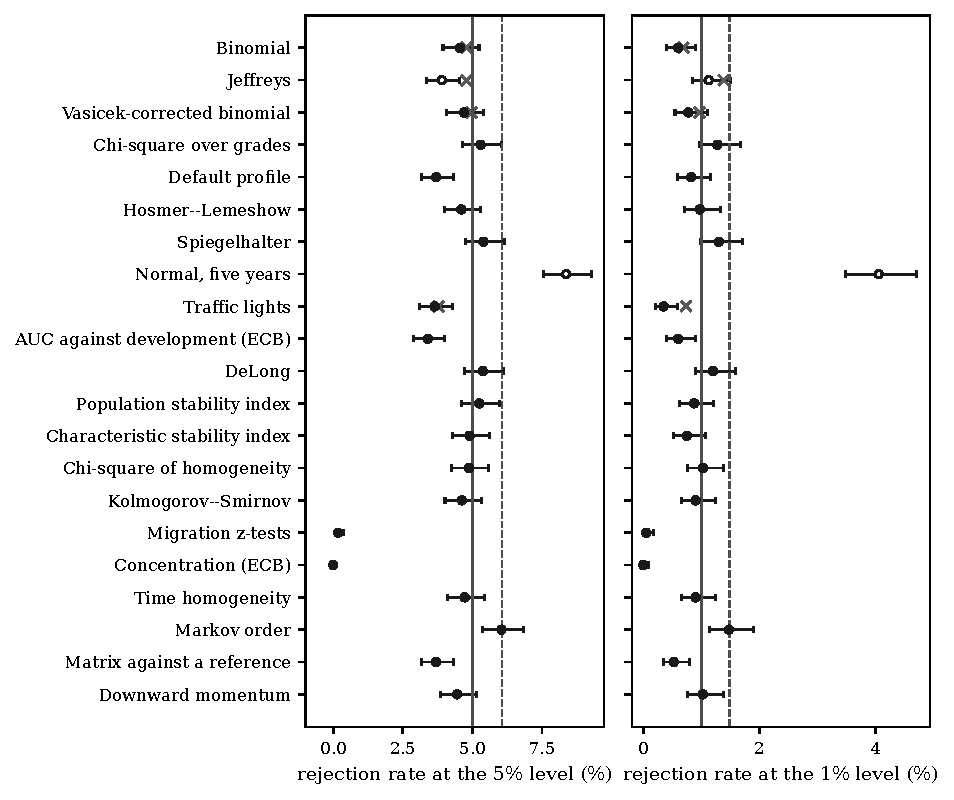
\includegraphics[width=\linewidth]{size_forest}
\caption{Measured size of the 21 credit-family tests at the 5\% level (left) and the 1\% level (right): the rate of the committed cell of 4,000 repetitions (circle) and the pooled rate of 200,000 repetitions (grey square), each with its Wilson 95\% interval, the level (solid line), the bound of the screen at 4,000 repetitions (dashed line), the exact rejection probability where it exists (cross), and open markers for the tests that do not hold their size on that evidence by \cref{def:holds}.}
\label{fig:size-forest}
\end{figure}

The other tests spread around their level and below it.
At 5\,\%, \nConsFive{} tests are conservative, with the whole Wilson interval below the level: the Jeffreys test at 5\,\% (exact \jeffExactFive\,\%), the default-profile test (\profileFive\,\%), the traffic-lights test (exact \tlLowerExact\,\%), the AUC test against the development AUC (\aucNullFive\,\%), the matrix test against a reference (\matFive\,\%), the migration z-tests (\migFive\,\%) and the concentration test (\hhiFive\,\%).
Two of these are conservative for a reason that is a property of the test and not of the sample: the migration z-tests control 42 cells at once with Holm's procedure, and the concentration statistic is bounded (\cref{prop:hhi}).
The binomial test is conservative because its count is discrete: its exact size at 5\,\% is \binExactFive\,\% and the simulated rate \binSimFive\,\% agrees with it.
The Markov-order test shows how the two rules part on one cell.
Its rate is \ordFive\,\% at 5\,\% against the bound of \boundFive\,\%, a margin of \markovBoundMargin\ points, so the screen passes it; but its Wilson interval, \ordLoFive\,\% to \ordHiFive\,\%, lies wholly above 5\,\%, and at 1\,\% its rate of \ordOne\,\% has an interval of \ordLoOne\,\% to \ordHiOne\,\%, wholly above 1\,\%, so by the definition it does not hold its size.
A run of 20,000 repetitions gives \ordTwentyK\,\% at 5\,\% with interval \ordTwentyKLo\,\% to \ordTwentyKHi\,\%, and the pool of the replication of \cref{sec:rs-seeds} \pooledOrd\,\%.
\Cref{fig:p-histograms} shows the p-values behind the rates: the binomial test has gaps where no count falls, the normal test piles its mass at small p-values, and the concentration test has all its mass at one, which is what a test that cannot reject looks like.

\begin{figure}[htbp]
\centering
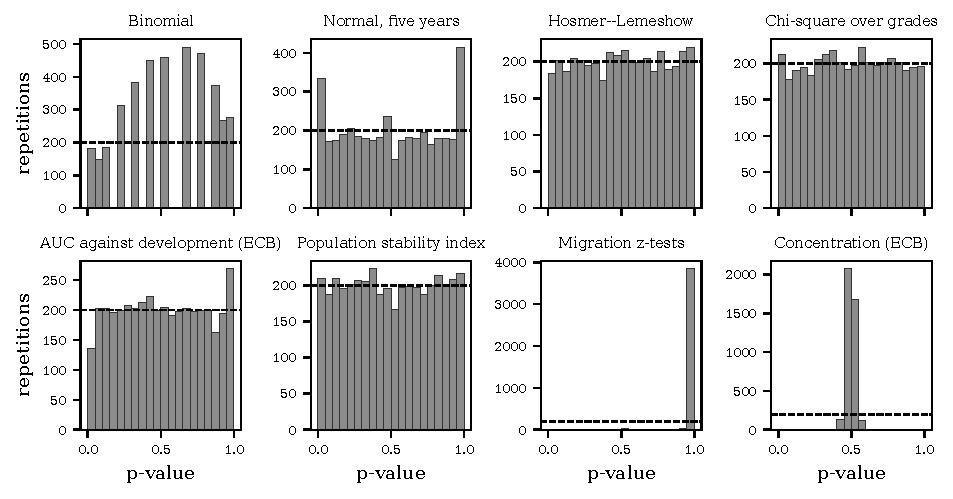
\includegraphics[width=\linewidth]{p_histograms}
\caption{Histograms of the p-values of eight tests under their null in 4,000 repetitions: a test that holds its size continuously has a flat histogram (dashed line), the discrete binomial test has empty bins, the normal test over five years has excess mass at small p-values, and the concentration test has all of its mass at one.}
\label{fig:p-histograms}
\end{figure}

\subsection{Settings that change a size}
\label{sec:rs-settings}

\Cref{tab:settings} lists the cells in which a setting of a test, and not a defect of the model, moves its size on the same generator.
Referring the Hosmer--Lemeshow statistic to two fewer degrees of freedom, as the original statistic does for a model fitted on the same sample, gives a size of \hlFitted\,\% at 5\,\% and \hlFittedOne\,\% at 1\,\% on a validation sample whose probabilities were not fitted on it, close to the \hlDofTheory\,\% of \cref{prop:reference}; with the degrees of freedom of the groups, the test has \hlFive\,\% and \hlOne\,\%.
The traffic-lights test measures \tlLowerExact\,\% exactly with the tie rule as printed and \tlUpperExact\,\% with the upper tie rule that the simulation of the Basel Committee must have used, so the rule that colours a year with exactly the expected number of defaults changes the size by two and a half points.
The chi-square test over grades rejects \chiThin\,\% at 5\,\% and \chiThinOne\,\% at 1\,\% when its best grade expects 0.6 defaults, above the bound at 1\,\%.
The AUC test against the development AUC rejects \aucDevOne\,\% at 5\,\% when the development AUC was estimated on a sample as large as the current one, against \aucDevOneExt\,\% when the variance of the development estimate is added, and \aucDevTheory\,\% is the prediction of \cref{prop:reference}.
The rules of thumb of the stability index, applied to two samples of 100 in which nothing changed, raise an alarm in \psiHundred\,\% of samples at 0.10 and \psiHundredTwentyFive\,\% at 0.25, against \psiHundredBench\,\% for its chi-square benchmark.

\begin{table*}[htbp]
\centering
\footnotesize
\caption{The settings of a test that change its measured size on the same null generator: Hosmer--Lemeshow with two fewer degrees of freedom, the traffic lights with the upper tie rule, a chi-square over a thin grade, the AUC test with an estimated development AUC and its extension, a longer run of the order test, and the PSI rules of thumb in samples of 100.}
\label{tab:settings}
\fitwidth{\begin{tabular}{p{2.4cm}p{4.6cm}rllcp{2.6cm}}
\toprule
Test & Setting & Reps & Size at 5\% [Wilson] & Size at 1\% & Exact 5\% / 1\% & Other rule \\
\midrule
Hosmer--Lemeshow & the same, with G $-$ 2 degrees of freedom (the model fitted on the same sample) & 4,000 & 10.97 [10.0, 12.0] & 3.38 & -- &  \\
Traffic lights & the upper tie rule WP14's simulation used & 4,000 & 6.35 [5.6, 7.1] & 1.40 & 6.03 / 1.13 &  \\
Chi-square over grades & a best grade expecting 0.6 defaults & 4,000 & 5.67 [5.0, 6.4] & 1.73 & -- &  \\
AUC against development (ECB) & the development AUC estimated on an equal sample (ECB form) & 4,000 & 11.58 [10.6, 12.6] & 4.52 & -- &  \\
AUC against development (ECB) & the same with the development AUC's variance added & 4,000 & 5.30 [4.6, 6.0] & 1.05 & -- &  \\
Markov order & the same chain, 20,000 repetitions: the order test's size measured to 0.15 points & 20,000 & 5.05 [4.8, 5.4] & 1.05 & -- &  \\
Population stability index & two samples of 100: the 0.10 and 0.25 rules of thumb & 4,000 & 6.98 [6.2, 7.8] & 2.05 & -- & PSI above 0.10: 85.0; above 0.25: 22.9 \\
\bottomrule
\end{tabular}}
\end{table*}


\subsection{Miscalibration and default clustering}
\label{sec:rs-defects}

\Cref{fig:power-calibration} shows the power of the nine calibration tests as the true probability of default rises above the one applied.
Each panel uses its own design, so the curves compare tests on the same panel and are not a ranking across panels.
On a portfolio of 5,000 obligors at 2\,\%, the binomial test rejects \binKOneTwoFive\,\% of samples when the true PD is 1.25 times the one applied (exact value \binKOneTwoFiveExact\,\%) and \binKOneFive\,\% at 1.5 times, and the Jeffreys test \jeffKOneTwoFive\,\% at 1.25.
On the obligor-level panel the Spiegelhalter test is the most powerful, with \spiKOneOne\,\% at 1.1 and \spiKOneTwoFive\,\% at 1.25 against \hlKOneOne\,\% and \hlKOneTwoFive\,\% for Hosmer--Lemeshow; on the panel of seven grades the chi-square test has \chiKOneOne\,\% and \chiKOneTwoFive\,\%.
Over five years the normal test rejects \normKOneTwoFive\,\% and the traffic-lights test \tlKOneTwoFive\,\% at 1.25.
Two curves show what correcting for a correlation costs and what a shape test cannot see.
The Vasicek-corrected binomial test, which assumes an asset correlation of 12\,\% that the generator does not have, rejects nothing at 1.25 or at 1.5 times and \vasKThree\,\% at three times (exact \vasKThreeExact\,\%).
The default-profile test rejects \profKThree\,\% when every probability of default is three times too low, its size, because it tests the shape of the curve and a uniform multiple leaves the shape unchanged.
The severity at which the curves of the tests that reach 80\,\% power cross it lies between \sSpi{} and \sHl{} times the PD applied for the seven tests of \cref{tab:power-summary} on these panels.

\begin{figure}[htbp]
\centering
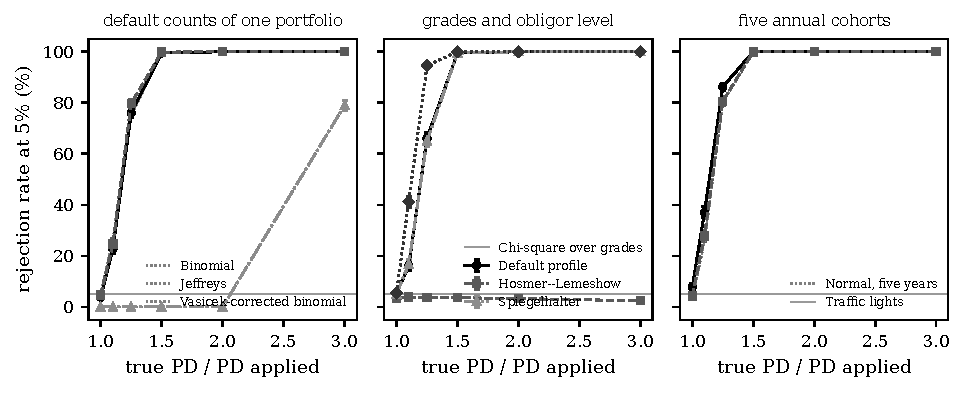
\includegraphics[width=\linewidth]{power_calibration}
\caption{Power at the 5\% level of the nine calibration tests against the ratio of the true probability of default to the one applied, in 2,000 repetitions per point with Wilson 95\% intervals; dotted lines are the exact rejection probabilities of the count tests and the traffic-lights test, which the simulated points follow.}
\label{fig:power-calibration}
\end{figure}

When the defaults are correlated and the probabilities of default are right, every rejection is a false alarm, and \cref{fig:clustering-size} shows how many.
At an asset correlation of 2\,\% the binomial test rejects \binRhoTwo\,\% of samples (exact \binRhoTwoExact\,\%), at 5\,\% it rejects \binRhoFive\,\% (exact \binRhoFiveExact\,\%), and at 10\,\% \binRhoOneZero\,\% (exact \binRhoOneZeroExact\,\%), against a level of 5\,\%, while the Vasicek-corrected test, whose assumed correlation is 12\,\%, holds its size near that correlation (\vasRhoOneZero\,\% at 10\,\%) and over-rejects beyond it (\vasRhoTwoZero\,\%, exact \vasRhoTwoZeroExact\,\%, at 20\,\%).
The tests built on grades and obligors fare worse: the chi-square test over grades rejects \chiRhoTwo\,\% at an asset correlation of 2\,\% and \chiRhoOneZero\,\% at 10\,\%, and Hosmer--Lemeshow \hlRhoTwo\,\% at 2\,\% and \hlRhoTwoZero\,\% at 20\,\%.
The normal test over five years goes the other way, from \normRhoZero\,\% at independence to \normRhoTwoZero\,\% at 20\,\%, because the year-to-year dispersion that it estimates absorbs the clustering.
A reader who sees a red light from a test that assumes independent defaults cannot tell a miscalibrated model from a correlated portfolio.

\begin{figure}[htbp]
\centering
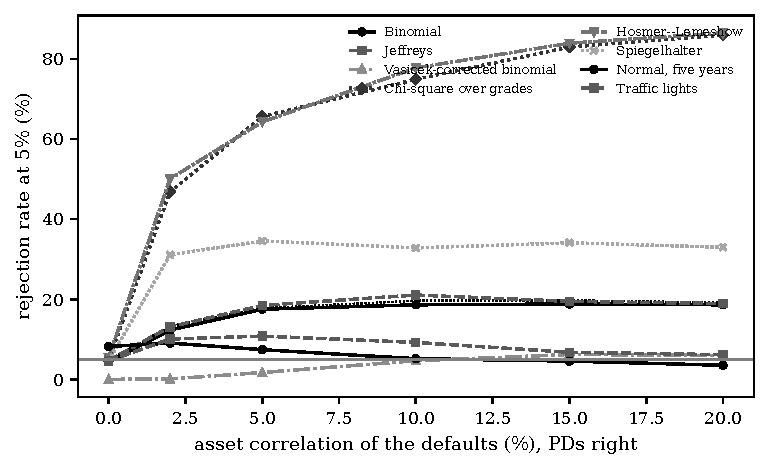
\includegraphics[width=0.85\linewidth]{clustering_size}
\caption{Rejection rate at 5\% of eight calibration tests when the probabilities of default are right and the defaults are correlated with the asset correlation on the horizontal axis, in 2,000 repetitions per point; the dotted line is the exact size of the binomial test, and every rejection above the level of 5\% is a false alarm.}
\label{fig:clustering-size}
\end{figure}

\subsection{Drift, discrimination, leakage and the rating system}
\label{sec:rs-stability}

\Cref{tab:power-summary} gives the power of the 17 tests along their ladders and \cref{fig:power-families} draws the curves of the other six defects.
For population drift of two samples of 1,000, the chi-square benchmark of the stability index has a power of \psiBenchZeroOne\,\% for a shift of 0.1 standard deviations and \psiBenchZeroTwo\,\% for 0.2; the chi-square test of homogeneity has \chiDriftZeroTwo\,\% at 0.2 and the Kolmogorov--Smirnov test \ksDriftZeroOne\,\% and \ksDriftZeroTwo\,\% at 0.1 and 0.2.
The fixed rules of thumb do not follow: at a shift of 0.2 the 0.10 rule alarms in \psiBandZeroOneAtZeroTwo\,\% and the 0.25 rule in \psiBandZeroTwoFiveAtZeroTwo\,\% of samples, and the 0.10 rule needs a shift of 0.3 to alarm in \psiBandZeroOneAtZeroThree\,\%.
The false alarm side of the same rules is in \cref{fig:psi-bands}: the measured rates of the printed study at the sample sizes in which nothing changed follow the asymptotic curve of \cref{prop:psi}.
A right model under a covariate shift stays calibrated, and the Hosmer--Lemeshow and Spiegelhalter tests reject \hlDriftZeroFive\,\% and \spiDriftZeroFive\,\% at a shift of 0.5 standard deviations, their size: drift and miscalibration are different questions.

\begin{figure}[htbp]
\centering
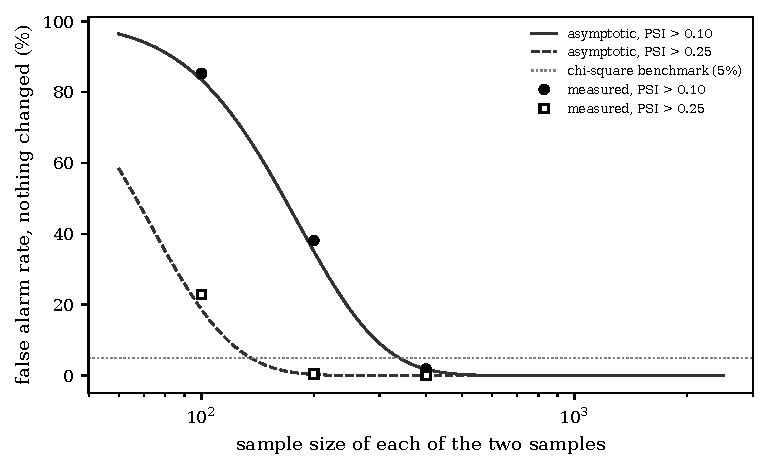
\includegraphics[width=0.85\linewidth]{psi_bands}
\caption{False alarm rate of the fixed bands of the population stability index when nothing changed, against the size of each of two samples: the asymptotic curves of the chi-square result for the bands 0.10 and 0.25, the 5\% of the chi-square benchmark, and the rates measured on the cells of the published study that the measurement reruns.}
\label{fig:psi-bands}
\end{figure}

For discrimination, with 150 defaulters, the ECB test against the development AUC rejects \ecbDropZeroTwo\,\% of samples for an AUC drop of two points, \ecbDropZeroFive\,\% for five and \ecbDropZeroEight\,\% for eight; DeLong's test, applied to a challenger whose AUC is lower by the same amount, rejects \delDropZeroTwo\,\% at two points and \delDropZeroFive\,\% at five, and it needs a drop of \delDropAtPower\ for 80\,\% power against \ecbDropAtPower\ for the ECB test.
Leakage of the outcome into a development feature is visible to the AUC test as a drop out of time, \leakAucZeroTwoFive\,\% at a shift of 0.25 and \leakAucZeroFive\,\% at 0.5, and almost invisible to the characteristic stability index of the leaked feature itself, which rejects \leakCsiZeroTwoFive\,\% at 0.25, \leakCsiOne\,\% at 1 and \leakCsiTwo\,\% at 2.
For the rating system, with 500 obligors per grade the migration z-tests reject \migROneFivenFiveZeroZero\,\% of samples when one cell is 1.5 times its closer neighbour, \migRTwonFiveZeroZero\,\% at twice and \migRThreenFiveZeroZero\,\% at three times; with 2,000 obligors the figures are \migROneFivenTwoZeroZeroZero\,\% at 1.5 and \migRTwonTwoZeroZeroZero\,\% at twice.
Swapping the default probabilities of two adjacent grades is seen by the default-profile test in \swapProfile\,\% of samples and by the chi-square test over grades in \swapChi\,\%.
The concentration test of the European Central Bank rejects \hhiPower\,\% of samples at every severity, including half of every grade's mass moved into the modal grade, where the chi-square test of homogeneity applied to the counts rejects \chiCountZeroZeroTwo\,\% at 2\,\% moved and \chiCountZeroZeroFive\,\% at 5\,\%.
\Cref{fig:hhi-bound} shows why: its statistic, computed exactly, stays below its critical value at every coefficient of variation.

\begin{table*}[htbp]
\centering
\footnotesize
\caption{Measured power at 5\%, in percent, of the 17 tests with a power curve at the six settings S1 to S6 of the ladder of the defect planted for each (2,000 repetitions per setting), and the setting at which the interpolated curve first reaches 80\% with the interval given by the Wilson limits of the points.}
\label{tab:power-summary}
\fitwidth{\begin{tabular}{llrrrrrrl}
\toprule
Test & Defect and ladder & S1 & S2 & S3 & S4 & S5 & S6 & Setting at 80\% power [95\%] \\
\midrule
Binomial & true PD / PD applied (1 to 3) & 3.8 & 22.8 & 76.0 & 99.6 & 100.0 & 100.0 & 1.29 [1.27, 1.31] \\
Jeffreys & true PD / PD applied (1 to 3) & 4.7 & 24.7 & 79.8 & 99.9 & 100.0 & 100.0 & 1.25 [1.25, 1.27] \\
Vasicek-corrected binomial & true PD / PD applied (1 to 3) & 0.0 & 0.0 & 0.0 & 0.0 & 0.0 & 79.0 & not reached \\
Chi-square over grades & true PD / PD applied (1 to 3) & 5.3 & 16.0 & 66.1 & 99.5 & 100.0 & 100.0 & 1.35 [1.34, 1.36] \\
Default profile & true PD / PD applied (1 to 3) & 3.3 & 3.9 & 3.8 & 3.6 & 3.2 & 2.4 & not reached \\
Hosmer--Lemeshow & true PD / PD applied (1 to 3) & 5.0 & 16.8 & 64.9 & 99.5 & 100.0 & 100.0 & 1.36 [1.35, 1.37] \\
Spiegelhalter & true PD / PD applied (1 to 3) & 5.3 & 41.2 & 94.6 & 100.0 & 100.0 & 100.0 & 1.21 [1.21, 1.21] \\
Normal, five years & true PD / PD applied (1 to 3) & 7.8 & 37.0 & 86.2 & 100.0 & 100.0 & 100.0 & 1.23 [1.23, 1.24] \\
Traffic lights & true PD / PD applied (1 to 3) & 4.3 & 27.8 & 80.6 & 100.0 & 100.0 & 100.0 & 1.25 [1.24, 1.26] \\
AUC against development (ECB) & AUC drop (0 to 0.08) & 2.9 & 11.6 & 25.4 & 46.2 & 81.5 & 99.1 & 0.0492 [0.0482, 0.0505] \\
DeLong & AUC drop (0 to 0.08) & 4.9 & 8.1 & 18.0 & 34.2 & 71.6 & 97.8 & 0.0596 [0.0578, 0.0614] \\
Population stability index & mean shift (standard deviations) (0 to 0.5) & 5.0 & 9.6 & 27.2 & 89.6 & 100.0 & 100.0 & 0.185 [0.182, 0.187] \\
Characteristic stability index & leak (shift of the feature for defaulters) (0 to 2) & 4.7 & 6.0 & 7.8 & 14.6 & 33.4 & 58.1 & not reached \\
Chi-square of homogeneity & mean shift (standard deviations) (0 to 0.5) & 4.6 & 9.3 & 26.2 & 88.5 & 100.0 & 100.0 & 0.186 [0.184, 0.189] \\
Kolmogorov--Smirnov & mean shift (standard deviations) (0 to 0.5) & 5.5 & 14.9 & 46.5 & 97.3 & 100.0 & 100.0 & 0.166 [0.164, 0.168] \\
Migration z-tests & planted cell / closer neighbour (1 to 4) & 0.1 & 1.3 & 7.9 & 55.5 & 99.7 & 100.0 & 2.55 [2.53, 2.58] \\
Concentration (ECB) & share moved into the modal grade (0 to 0.5) & 0.0 & 0.0 & 0.0 & 0.0 & 0.0 & 0.0 & not reached \\
\bottomrule
\end{tabular}}
\end{table*}


\begin{figure}[htbp]
\centering
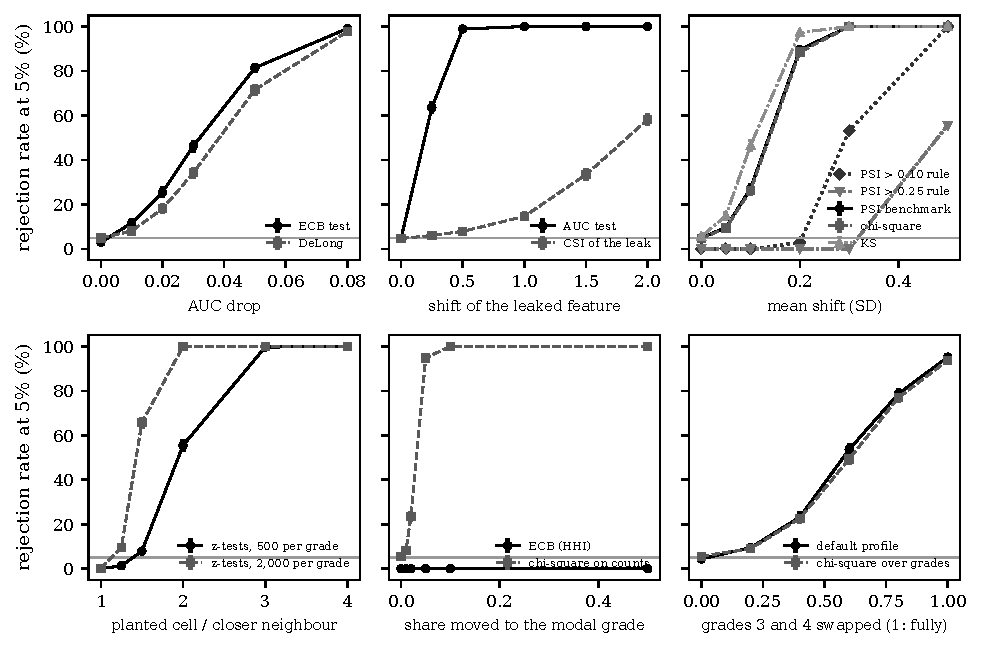
\includegraphics[width=\linewidth]{power_families}
\caption{Power at 5\% against the planted defect of the tests of discrimination decay, leakage, drift, broken monotonicity of the migrations, concentration and swapped grades, with Wilson 95\% intervals in 2,000 repetitions per point; drift also shows the rules of thumb PSI above 0.10 and above 0.25, which never reach the power of the benchmark.}
\label{fig:power-families}
\end{figure}

\begin{figure}[htbp]
\centering
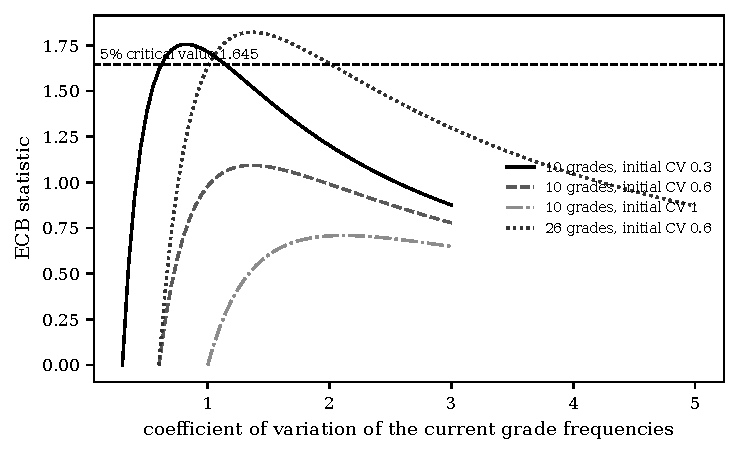
\includegraphics[width=0.85\linewidth]{hhi_bound}
\caption{The concentration statistic of the European Central Bank as a function of the current coefficient of variation of the grade frequencies, computed exactly for 10 grades with initial coefficients of variation 0.3, 0.6 and 1 and for 26 grades with 0.6; only the curves that rise above the dashed critical value of 1.645 can reject at 5\%.}
\label{fig:hhi-bound}
\end{figure}

Of the \nPowerTests{} curves, \nReach{} reach 80\,\% on their ladder.
The four that do not are the Vasicek-corrected binomial test (\vasKThree\,\% at the top of its ladder, within the Monte Carlo error of 80\,\%), the default-profile test against a uniform multiple of the probabilities, the characteristic stability index against a leak, and the concentration test.
For the ones that do, the severity at which the curve crosses 80\,\% is in \cref{tab:power-summary}: for example an AUC drop of \ecbDropAtPower, a mean shift of \sPsi, \sChiStab{} and \sKs{} standard deviations for the benchmark of the stability index, the chi-square test of homogeneity and the Kolmogorov--Smirnov test, and a planted migration cell \sMig{} times its closer neighbour for 500 obligors per grade.

\subsection{The instrument: exact values, published studies and reproduction}
\label{sec:rs-instrument}

The exact rejection probabilities of \nExactRows{} rows give \nExactCmp{} comparisons with the simulated rates at two levels, and all \nAgree{} agree within 3.29 standard errors by \eqref{eq:agree}; the largest absolute $z$ is \zMaxAbs.
Over the \nExactNondeg{} comparisons whose exact probability lies between 0.5\,\% and 99.5\,\%, where a rate can differ from it, the mean of $z$ is \zMean{} and its standard deviation \zSd, above one; the two levels of a row share their draws, so the values are not independent and their standard deviation is less precise than for independent values, and none exceeds 3.29.
A routine that calls no function of the engine and recomputes the exact rejection probability of the binomial test from the configuration of each generator reproduces \nBinRecon{} of the committed exact values to $\binReconMax$.
No power curve falls by more than 3.29 combined standard errors between neighbouring severities: \nMonoViol{} violations in \nMonoPairs{} adjacent pairs, against the expected 0.1 of \cref{sec:th-monotone}.

The reruns of the published studies are in \cref{tab:reproductions} and \cref{fig:reproductions}.
The rerun agrees with \wpAgree{} of the \wpTotal{} cells of the normal and traffic-lights tests of the Basel Committee at \wpRuns{} runs; the one cell that does not, the traffic-lights test in the scenario labelled DV\_LV at the 0.1\,\% level, is printed as \wpOffPub\,\% and measured as \wpOffMeas\,\%.
It agrees with \ynAgree{} of the \ynTotal{} cells of the stability study at \ynRuns{} runs; the harness sits slightly above the printed rates, with a mean $z$ of $+\ynMeanZ$ over the \ynInterior{} cells whose printed rate is strictly between 0 and 1.
The nested-model rate of the DeLong test is \demlerMeasured\,\% in \demlerRuns{} runs against the printed \demlerPublished\,\%.
Every one of the \nReproTotal{} committed null cells reproduces exactly: the counts of rejections, at both levels, and the number of undefined results equal the committed ones when the cell is rerun from its configuration and its seed.
The estimators that the harness also measures agree: the AUC of 4,000 binormal samples has a normal interval that covers \aucCover\,\% of the time (Monte Carlo standard error \aucCoverMcse\,\%), and the standard error of the ECB formula differs from the empirical one by $\aucSeRel\,\%$.

\begin{table*}[htbp]
\centering
\footnotesize
\caption{The three published simulation studies rerun by the measurement: the runs of the study and of the rerun, the cells whose printed rate agrees with the measured one within 3.29 pooled standard errors, the mean z of the differences, and each cell that disagrees.}
\label{tab:reproductions}
\fitwidth{\begin{tabular}{p{4.2cm}rrrp{5.3cm}}
\toprule
Published study & Runs: printed / ours & Cells agreeing & Mean z & Cells that disagree \\
\midrule
BCBS WP14 Tables 7 and 8: the normal and traffic-lights tests & 25,000 / 25,000 & 143 of 144 & -0.11 & DV\_LV, traffic, 0.001: printed 0.955, measured 0.9436 \\
Yurdakul and Naranjo (2020) Table 4: the PSI's rules and benchmark & 10,000 / 10,000 & 50 of 54 & +0.67 & m 100, n 400, shift 0.25 SD, PSI $>$ 0.10: printed 0.834, measured 0.8522; m 100, n 400, shift 0.5 SD, PSI $>$ 0.25: printed 0.787, measured 0.8098; m 200, n 200, shift 0 SD, chi-square: printed 0.057, measured 0.0688; m 200, n 400, shift 0.5 SD, PSI $>$ 0.25: printed 0.72, measured 0.7421 \\
Demler, Pencina and D'Agostino (2012): DeLong on nested models & 1,000 / 1,000 & 1 of 1 & +0.58 & none \\
\bottomrule
\end{tabular}}
\end{table*}


\begin{figure}[htbp]
\centering
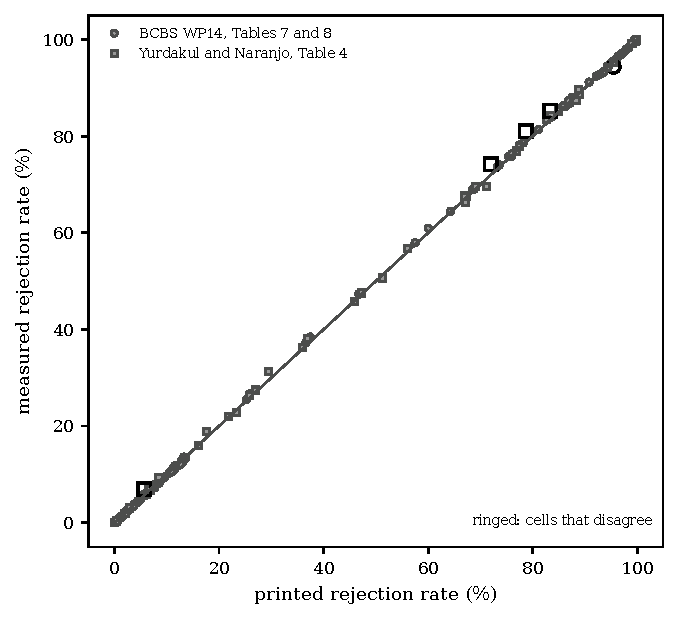
\includegraphics[width=0.7\linewidth]{reproductions}
\caption{Printed rejection rate against the rate measured by the rerun, for the 144 cells of the Basel Committee's study of the normal and traffic-lights tests and the 54 cells of the stability index study; the diagonal is agreement and the ringed points are the cells that do not agree within 3.29 pooled standard errors.}
\label{fig:reproductions}
\end{figure}

\subsection{Replication across seeds}
\label{sec:rs-seeds}

\Cref{tab:seed-replication} and \cref{fig:seed-spread} report the \nBlocks{} independent blocks of each test.
The Monte Carlo standard error is calibrated: the standard deviation of the block rates over the binomial standard error, $\kappa$ of \eqref{eq:kappa}, has a mean of \sdRatioMean{} over tests and levels, with a range from \sdRatioMin{} to \sdRatioMax{}, as fifty blocks allow.
The pooled sizes sort the tests into three groups: \nWithin{} lie within the level (the pooled rate does not exceed it at either level), \nOver{} lie above it (the lower Wilson limit of the pooled rate exceeds the level at one level), and \nNeither{} are in neither, with a pooled rate slightly above the level at one level and an interval that includes it (the chi-square test of homogeneity and the downward-momentum test).
The tests of the third group hold their size by \cref{def:holds}, so that the tests of the first and third groups, \nHold{} in all, hold their size on the pool and the \nOver{} of the second do not.
Among the \nOver{} are the two tests that the committed cells flag by the screen, and \nSmallOver{} others whose excess, at the level that places them above, is small: the stability index at \pooledPsi\,\% at 5\,\%, Hosmer--Lemeshow at \pooledHl\,\% (and \pooledHlOne\,\% at 1\,\%), the Spiegelhalter test, the Markov-order test and the chi-square test over grades (respectively \pooledSpi\,\%, \pooledOrd\,\% and \pooledChi\,\% at 5\,\%), DeLong at \pooledDel\,\% at 5\,\% and the characteristic stability index at \pooledCsiOne\,\% at 1\,\% (its 5\,\% rate, \pooledCsi\,\%, has an interval that includes the level); the excesses range from \smallExcMin{} to \smallExcMax{} points, below what a cell of \nNullReps{} repetitions can resolve (\detIntFiveFour{} points at 5\,\%).
The judgement of the committed cell equals that of the pool, both by \cref{def:holds}, for \nVerdictAgree{} of the \nTests{} tests and differs for \nVerdictDisagree{}, the tests that the pool shows above their level and the cell does not; by the screen the figures are \nVerdictAgreeRule{} and \nVerdictDisagreeRule{}.
The normal test pools to \pooledNorm\,\% and the Jeffreys test to \pooledJeffOne\,\% at 1\,\%, the exact value.

\begin{table*}[htbp]
\centering
\footnotesize
\caption{Fifty independent blocks of 4,000 repetitions (200,000 in all) for each of the 21 tests: the committed cell, the pooled rate with its Wilson interval, the standard deviation of the block rates beside the binomial standard error at 5\%, the share of blocks flagged by the one-sided bound and by the rule that a rate above the level is oversized, and the judgement of the committed cell and of the pool.}
\label{tab:seed-replication}
\fitwidth{\begin{tabular}{lrlcrrlcc}
\toprule
Test & Cell 5\% & Pooled 5\% [Wilson] & SD / SE of blocks & Flagged: bound / naive (\%) & Cell 1\% & Pooled 1\% [Wilson] & Cell holds & Pooled holds \\
\midrule
Binomial & 4.55 & 4.81 [4.72, 4.91] & 0.33 / 0.34 & 0 / 26 & 0.60 & 0.66 [0.62, 0.69] & yes & yes \\
Jeffreys & 3.90 & 4.71 [4.62, 4.81] & 0.32 / 0.34 & 0 / 18 & 1.12 & 1.38 [1.33, 1.43] & no & no \\
Vasicek-corrected binomial & 4.70 & 4.92 [4.82, 5.01] & 0.42 / 0.34 & 0 / 44 & 0.78 & 1.00 [0.95, 1.04] & yes & yes \\
Chi-square over grades & 5.30 & 5.15 [5.06, 5.25] & 0.37 / 0.35 & 2 / 64 & 1.27 & 1.21 [1.16, 1.26] & yes & no \\
Default profile & 3.70 & 4.05 [3.97, 4.14] & 0.29 / 0.31 & 0 / 0 & 0.83 & 0.76 [0.72, 0.80] & yes & yes \\
Hosmer--Lemeshow & 4.60 & 5.17 [5.08, 5.27] & 0.31 / 0.35 & 0 / 68 & 0.97 & 1.26 [1.21, 1.31] & yes & no \\
Spiegelhalter & 5.40 & 5.15 [5.06, 5.25] & 0.32 / 0.35 & 0 / 66 & 1.30 & 1.10 [1.06, 1.15] & yes & no \\
Normal, five years & 8.38 & 7.99 [7.87, 8.11] & 0.40 / 0.43 & 100 / 100 & 4.05 & 3.56 [3.48, 3.64] & no & no \\
Traffic lights & 3.65 & 3.81 [3.73, 3.90] & 0.30 / 0.30 & 0 / 0 & 0.35 & 0.73 [0.70, 0.77] & yes & yes \\
AUC against development (ECB) & 3.40 & 4.00 [3.91, 4.08] & 0.28 / 0.31 & 0 / 0 & 0.60 & 0.63 [0.59, 0.66] & yes & yes \\
DeLong & 5.38 & 5.13 [5.03, 5.23] & 0.31 / 0.35 & 0 / 68 & 1.20 & 1.03 [0.99, 1.08] & yes & yes \\
Population stability index & 5.25 & 5.29 [5.19, 5.38] & 0.43 / 0.35 & 4 / 78 & 0.88 & 1.10 [1.06, 1.15] & yes & no \\
Characteristic stability index & 4.90 & 5.09 [5.00, 5.19] & 0.35 / 0.35 & 2 / 60 & 0.75 & 1.05 [1.00, 1.09] & yes & yes \\
Chi-square of homogeneity & 4.88 & 5.00 [4.91, 5.10] & 0.39 / 0.34 & 0 / 48 & 1.03 & 1.00 [0.96, 1.04] & yes & yes \\
Kolmogorov--Smirnov & 4.62 & 4.87 [4.78, 4.96] & 0.30 / 0.34 & 0 / 30 & 0.90 & 0.99 [0.95, 1.03] & yes & yes \\
Migration z-tests & 0.18 & 0.11 [0.10, 0.13] & 0.05 / 0.05 & 0 / 0 & 0.05 & 0.02 [0.02, 0.03] & yes & yes \\
Concentration (ECB) & 0.00 & 0.00 [0.00, 0.00] & 0.00 / 0.00 & 0 / 0 & 0.00 & 0.00 [0.00, 0.00] & yes & yes \\
Time homogeneity & 4.72 & 4.35 [4.26, 4.44] & 0.31 / 0.32 & 0 / 0 & 0.90 & 0.78 [0.74, 0.81] & yes & yes \\
Markov order & 6.05 & 5.15 [5.05, 5.25] & 0.35 / 0.35 & 0 / 62 & 1.47 & 1.11 [1.07, 1.16] & yes & no \\
Matrix against a reference & 3.70 & 3.34 [3.27, 3.42] & 0.30 / 0.28 & 0 / 0 & 0.53 & 0.62 [0.58, 0.65] & yes & yes \\
Downward momentum & 4.45 & 4.98 [4.89, 5.08] & 0.35 / 0.34 & 0 / 46 & 1.03 & 1.01 [0.97, 1.06] & yes & yes \\
\bottomrule
\end{tabular}}
\end{table*}


\begin{figure}[htbp]
\centering
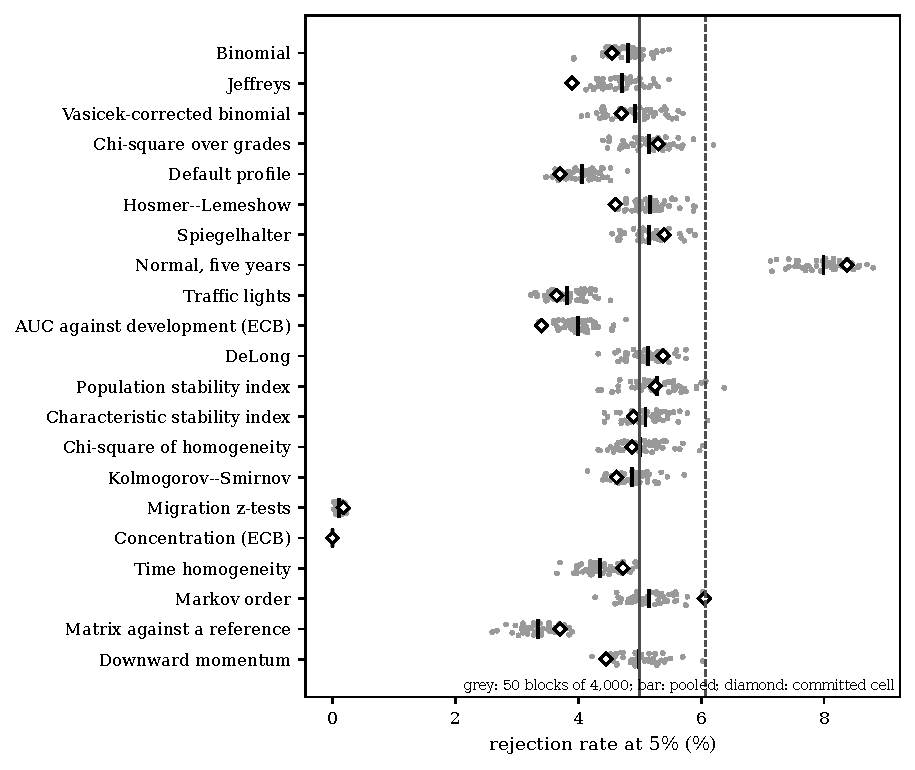
\includegraphics[width=\linewidth]{seed_spread}
\caption{Rejection rate at 5\% of each of the 21 tests in 50 independent blocks of 4,000 repetitions (grey points), the pooled rate (vertical bar) and the committed cell (diamond); the solid line is the level and the dashed line the bound of a cell of 4,000 repetitions.}
\label{fig:seed-spread}
\end{figure}

\subsection{The 21 tests outside the credit families}
\label{sec:extension}

The engine registers \nExtTests{} further p-value tests of counterparty credit risk, provisioning, loss given default, market risk, portfolio credit risk, fairness and machine learning, which it measures through \nStudies{} named studies, each with a generator of the null and one stated alternative.
\Cref{tab:extension} and \cref{fig:extension} give the size of each at 4,000 repetitions and its power against its one alternative at 2,000.
By \cref{def:holds} on cells of \nNullReps{} repetitions, \nExtHold{} of the \nExtTests{} tests hold their size at both levels, and \nStudiesHold{} of the \nStudies{} studies; the screen passes \nExtHoldRule{} tests and \nStudiesHoldRule{} studies.
The \nStudiesNotHold{} studies that do not hold are the independence test and the conditional-coverage test of Christoffersen, at the series length of 1,500 days at 5\,\% (the independence test rejects \chrIndFive\,\% at 5\,\% and \chrIndOne\,\% at 1\,\%, and the conditional-coverage test \chrCcFive\,\% at 5\,\%), the calibration of the loss given default over time (\lgdTimeOne\,\% at 1\,\%), the convergence of the Monte Carlo quantile, whose excess the engine documents (\mcConvFive\,\% at 5\,\%), and the unconditional test of Du and Escanciano (\duUncondFive\,\% at 5\,\%).
These are single cells without a replication, so each judgement carries the resolution of \detIntFiveFour{} points, and at most about \expFalseAboveExt{} of the 25 studies would be shown above their level by chance if every study had exactly its level.
Among these tests are the residual test of \citet{mcneil2000}, the duration test of \citet{christoffersen2004}, the expected-shortfall tests of \citet{acerbi2014} and \citet{du2017}, the dynamic quantile test of \citet{engle2004}, and the recursion for CreditRisk+ \citep{haaf2004} that the study compares with a Monte Carlo run.
At 5\,\%, \nExtCons{} studies are conservative, with the whole interval below the level.
Against its stated alternative the power at 5\,\% runs from \extPowMin\,\% to \extPowMax\,\% with a median of \extPowMed\,\%; \extAboveBar{} studies reach 80\,\% and \extBelowHalf{} detect their alternative less than half of the time.
These alternatives are the engine's choices, one departure for each test, and the powers are not comparable across tests.

\begin{table}[htbp]
\centering
\footnotesize
\caption{The 25 named studies of the 21 tests outside the credit families: the measured size at 5\% and 1\% (4,000 repetitions) on the null of each study, whether both sizes lie within the one-sided bound, and the power at 5\% against the one alternative the study states (2,000 repetitions), in percent.}
\label{tab:extension}
\fitwidth{\begin{tabular}{p{7.4cm}rrcr}
\toprule
Study & Size at 5\% & Size at 1\% & Holds & Power at 5\% $\pm$ SE \\
\midrule
PFE exceedance back-test, PFE at 95\%, 1,000 dates & 5.25 & 1.23 & yes & 72.5 $\pm$ 1.0 \\
IFRS 9 stage-migration back-test, three stages, 4,000, 1,500 and 500 accounts & 4.75 & 1.10 & yes & 74.9 $\pm$ 1.0 \\
LGD calibration by segment, one segment, 250 workouts & 4.67 & 0.78 & yes & 82.4 $\pm$ 0.9 \\
LGD calibration over time, five default years, 60 workouts each & 5.12 & 1.47 & yes & 57.6 $\pm$ 1.1 \\
Downturn LGD coverage, 150 downturn workouts, estimate 0.45 & 5.42 & 1.25 & yes & 67.1 $\pm$ 1.1 \\
McNeil--Frey residual test, 2,500 days at 5\%, 125 exceedances expected & 3.57 & 0.43 & yes & 93.2 $\pm$ 0.6 \\
Tail back-test (LHP quantile), 60 years at the 95\% level & 3.57 & 1.15 & yes & 30.1 $\pm$ 1.0 \\
Tail back-test (LHP quantile), 250 years at the 99\% level & 4.20 & 0.35 & yes & 96.0 $\pm$ 0.4 \\
Monte Carlo quantile convergence, 20,000 scenarios, the 99\% quantile of the LHP loss rate & 5.88 & 1.32 & yes & 74.6 $\pm$ 1.0 \\
CreditRisk+ recursion against Monte Carlo, 2,000 scenarios, 400 obligors in five exposure bands & 3.02 & 0.73 & yes & 55.8 $\pm$ 1.1 \\
Two-proportion z (fairness), 2,000 applicants, two groups & 5.47 & 0.92 & yes & 99.0 $\pm$ 0.2 \\
Fisher exact (fairness), 2,000 applicants, two groups & 4.52 & 1.05 & yes & 98.6 $\pm$ 0.3 \\
Kupiec proportion of failures, 1,500 days at 5\% & 4.80 & 0.83 & yes & 69.3 $\pm$ 1.0 \\
Christoffersen independence, 1,500 days at 5\% & 5.67 & 1.52 & \textbf{no} & 87.5 $\pm$ 0.7 \\
Christoffersen conditional coverage, 1,500 days at 5\% & 6.90 & 1.43 & \textbf{no} & 81.2 $\pm$ 0.9 \\
Duration test, 400 days at 5\% & 3.92 & 0.00 & yes & 59.7 $\pm$ 1.1 \\
Acerbi--Sz\'ekely ES test, 250 days at 2.5\% & 4.92 & 1.20 & yes & 89.4 $\pm$ 0.7 \\
Du--Escanciano, unconditional, 2,000 days at 10\% & 5.78 & 1.38 & yes & 56.5 $\pm$ 1.1 \\
Du--Escanciano, conditional, 2,000 days at 10\% & 4.85 & 1.10 & yes & 73.2 $\pm$ 1.0 \\
Dynamic quantile test, 1,500 days at 5\% & 4.00 & 0.00 & yes & 71.0 $\pm$ 1.0 \\
Dynamic quantile test, 250 days at 1\% & 4.42 & 0.00 & yes & 14.0 $\pm$ 0.8 \\
Dynamic quantile test, 250 days at 2.5\% & 4.23 & 0.00 & yes & 23.8 $\pm$ 1.0 \\
Dynamic quantile test, 750 days at 1\% & 3.43 & 0.00 & yes & 26.2 $\pm$ 1.0 \\
Shift resilience (ML), 2,000 development rows, a quarter worst-subsample share & 4.95 & 0.00 & yes & 97.0 $\pm$ 0.4 \\
Conformal coverage (ML), 2,000 test rows, 90\% coverage & 4.60 & 0.97 & yes & 100.0 $\pm$ 0.0 \\
\bottomrule
\end{tabular}}
\end{table}


\begin{figure}[htbp]
\centering
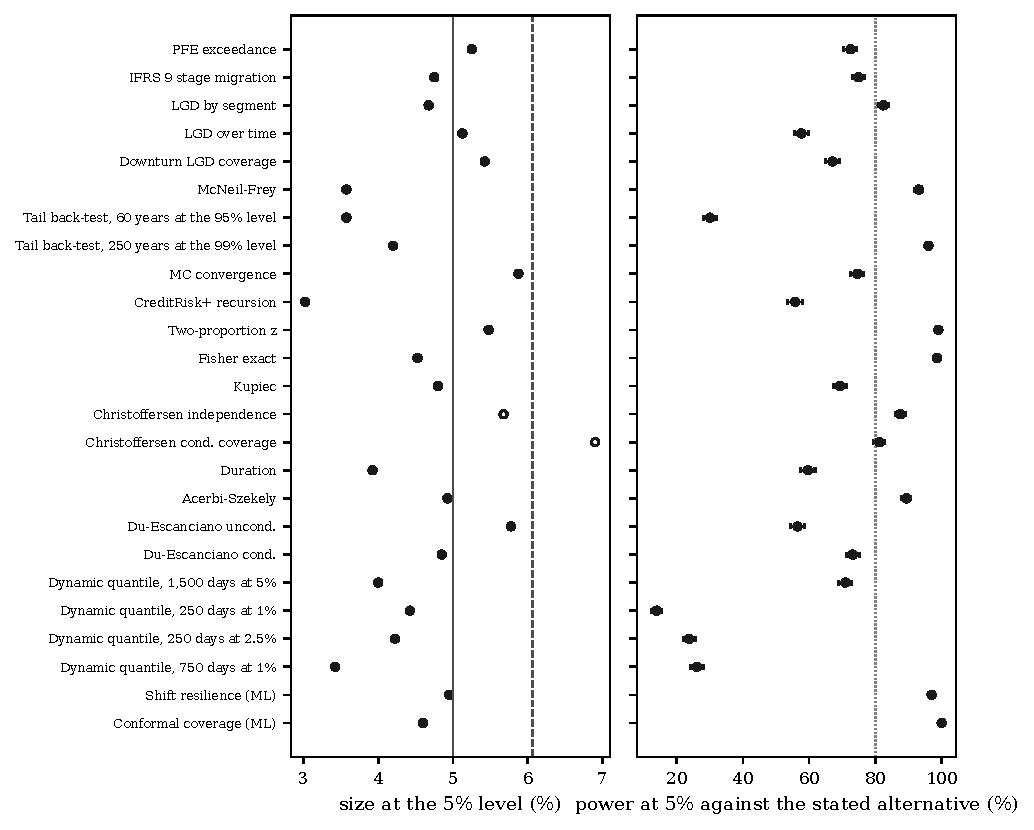
\includegraphics[width=\linewidth]{extension}
\caption{Size at 5\% (left, with the level as a solid line and the one-sided bound as a dashed line) and power at 5\% against the one alternative that each study states (right, with Wilson 95\% intervals and a dotted line at 80\%) for the 25 studies of the 21 tests outside the credit families.}
\label{fig:extension}
\end{figure}

\subsection{Whether each prediction held}
\label{sec:rs-hypotheses}

\Cref{tab:outcomes} reports the eight predictions of \cref{tab:predictions} against their criteria.
Five held and three are refuted.
P2 is refuted: \nNotHoldCellDef{} of the \nTests{} tests do not hold their size on the committed cells and \nNotHold{} do not on the pool.
P7 is refuted: the judgement of one cell of \nNullReps{} repetitions differs from that of the pool for \nVerdictDisagree{} tests.
P8 is refuted: \nNoReach{} of the \nPowerTests{} power curves do not reach 80\,\% on their ladder. The three refutations have three different causes. P2 fails because of \nNotHold{} tests on the pool: two with the largest excess and two different mechanisms, a Bayesian posterior used as a frequentist test of a discrete count and an aggregate over five years whose oversizing the simulation of the Basel Committee also shows, and \nSmallOver{} more with small excesses, of which the Markov-order test is already shown by the committed cell. P7 fails because the resolution of a cell is coarser than the excesses that \nVerdictDisagree{} tests have, of \smallExcMin{} to \smallExcMax{} points. P8 fails because four tests do not respond to the defect planted for them within the ladder, which is a statement about the pair of test and ladder.

\begin{table}[htbp]
\centering
\footnotesize
\caption{Outcome of each prediction of the measurement against its criterion, with the numbers from the committed documents and the experiments; P2, P7 and P8 are refuted, the other five hold.}
\label{tab:outcomes}
\fitwidth{\begin{tabular}{p{0.8cm}p{5.4cm}p{6.5cm}p{1.4cm}}
\toprule
ID & Criterion & Measured & Outcome \\
\midrule
P1 & 21 sizes, 17 curves, every rate with its error & \nSims{} simulations, \nRates{} rates, all with standard error and Wilson interval; 4 transition tests with a size only & held \\
P2 & 21 of 21 tests hold their size, by \cref{def:holds} & \nHoldCellDef{} of 21 hold on the cells of 4,000 repetitions (\nHoldCellRule{} pass the screen) and \nHold{} on the pool of 200,000; Jeffreys at 1\,\% (exact \jeffExactOne\,\%) and the normal test over five years (\normFive\,\%) do not hold on either & refuted \\
P3 & all exact comparisons agree & \nAgree{} of \nExactCmp{}, largest $|z|$ \zMaxAbs & held \\
P4 & at least 143 of 144, 48 of 54, and the nested-model rate & \wpAgree{} of \wpTotal{}, \ynAgree{} of \ynTotal{}, \demlerMeasured\,\% against \demlerPublished\,\% & held \\
P5 & no fall of more than 3.29 combined standard errors & \nMonoViol{} of \nMonoPairs{} pairs & held \\
P6 & every committed count reproduces & \nReproduced{} of \nReproTotal{} cells exact & held \\
P7 & one cell and the pool judge every test alike, by \cref{def:holds} & \nVerdictAgree{} of 21 agree (\nVerdictAgreeRule{} by the screen) & refuted \\
P8 & every power curve reaches 80\,\% & \nReach{} of \nPowerTests{} reach it & refuted \\
\bottomrule
\end{tabular}}
\end{table}

\section{Ablation}
\label{sec:ablation}

The protocol has four components that a different choice could replace, and each earns its place only if removing it changes a result.
\Cref{tab:ablation} summarises what each removal changes, with the numbers of the experiments of \cref{sec:experimental-design}; the four subsections give the evidence.

\begin{table}[htbp]
\centering
\footnotesize
\caption{Ablation of the protocol: the component removed, what replaces it, the measure on which the two are compared, and its value with and without the component, from the exact coverage calculation, the committed counts, the fifty-block replication and the exact calculations of the instrument experiment.}
\label{tab:ablation}
\fitwidth{\begin{tabular}{p{2.4cm}p{2.5cm}p{4.6cm}p{2.2cm}p{2.2cm}}
\toprule
Component & Replaced by & Measure & With & Without \\
\midrule
Wilson interval & normal approximation & coverage of the 95\,\% interval at a true rate of 0.1\,\% in 4,000 repetitions & \covWilsonThousandth\,\% & \covWaldThousandth\,\% \\
Wilson interval & normal approximation & exact values inside the interval, of \nExactNondeg{} comparisons & \ivWilsonNd{} & \ivWaldNd{} \\
Wilson interval & normal approximation & upper limit for a rate of 0 in 4,000 repetitions (the concentration test) & \hhiWilsonHi\,\% & 0\,\% \\
Screen and definition & rate above the level & share of cells flagged, tests within the level, 4,000 repetitions & \flWithinBoundFour\,\% (screen), \flWithinIntFour\,\% (definition) & \flWithinNaiveFour\,\% \\
Screen and definition & rate above the level & share of cells flagged, tests above the level, 4,000 repetitions & \flOverBoundFour\,\% (screen), \flOverIntFour\,\% (definition) & \flOverNaiveFour\,\% \\
Exact value beside the rate & simulation alone & probability of detecting a generator whose PD is 5\,\% too high & \agFailFivePercent\,\% & none \\
Exact value beside the rate & simulation alone & Jeffreys test at 1\,\%: excess over the level seen by one cell & decided (\jeffExactOne\,\%) & \jeffDetect\,\% \\
4,000 repetitions & 1,000 & excess over 5\,\% seen with probability 0.8 (points) & \detFiveFour & \detFiveThousand \\
4,000 repetitions & 20,000 & excess over 5\,\% seen with probability 0.8 (points) & \detFiveFour & \detFiveTwentyK \\
\bottomrule
\end{tabular}}
\end{table}

\subsection{The interval of a rate}
\label{sec:ab-interval}

\Cref{tab:interval-coverage} and \cref{fig:interval-coverage} give the exact coverage of five nominal 95\,\% intervals for a rejection rate measured in 4,000 repetitions.
Above a true rate of 1\,\% the intervals differ by about one point of coverage at most: at 5\,\% the Wilson, Agresti--Coull and Clopper--Pearson intervals cover \covWilsonFive\,\%, the Jeffreys interval \covJefFive\,\% and the normal approximation \covWaldFive\,\%.
Below it they separate.
At a true rate of 0.1\,\%, where the size of a conservative test sits, the normal approximation covers \covWaldThousandth\,\%, the Wilson interval \covWilsonThousandth\,\%, the Clopper--Pearson and Jeffreys intervals \covCPThousandth\,\% and the Agresti--Coull interval \covACThousandth\,\%, so that the poor coverage of the normal approximation at small proportions that \citet{brown2001} describe is reproduced at the rates of this measurement.
On the committed rows that carry an exact value, the five intervals contain the exact probability in \ivWaldNd{} to \ivWilsonNd{} of the \nExactNondeg{} comparisons that are not at the edge of the unit interval, against the \nExactNondeg{} times 0.95 that nominal coverage would give; the shortfall is small, consistent with the spread of $z$ above one, and it does not separate the methods.
Over all \nExactCmp{} comparisons, including those whose exact value is at the edge of the unit interval, the Wilson, Jeffreys, Agresti--Coull and Clopper--Pearson intervals contain the exact value in \ivWilsonAll{}, \ivJefAll{}, \ivACAll{} and \ivCPAll{}, and the normal approximation in \ivWaldAll{}, because its interval has zero width at a rate of 0 or 1 and so excludes an exact value that is not exactly 0 or 1.
The practical difference is at a rate of zero.
The concentration test rejects in none of 4,000 repetitions, and the normal-approximation interval of that result has zero width, a claim of no uncertainty, while the Wilson interval has an upper limit of \hhiWilsonHi\,\%.
The Wilson interval is therefore adequate everywhere the measurement needs it, and necessary only for the conservative tests; the choice among the score, exact and Jeffreys intervals changes no judgement.

\begin{table}[htbp]
\centering
\footnotesize
\caption{Exact coverage, in percent, of five nominal 95\% intervals for a rejection rate measured in 4,000 repetitions, at five true rejection probabilities, and the number of the committed exact rejection probabilities that fall inside the interval of the simulated rate.}
\label{tab:interval-coverage}
\fitwidth{\begin{tabular}{lrrrrrcc}
\toprule
Interval & $r=0.1$\% & 0.5\% & 1\% & 5\% & 50\% & Exact value inside (63) & Inside (all 94) \\
\midrule
Wald & 90.6 & 94.8 & 94.4 & 94.9 & 94.8 & 56 of 63 & 68 of 94 \\
Wilson & 93.1 & 94.5 & 95.4 & 95.4 & 94.8 & 57 of 63 & 87 of 94 \\
Agresti--Coull & 97.9 & 94.5 & 95.4 & 95.4 & 94.8 & 57 of 63 & 88 of 94 \\
Clopper--Pearson & 96.0 & 95.7 & 96.2 & 95.4 & 95.2 & 57 of 63 & 88 of 94 \\
Jeffreys & 96.0 & 95.7 & 94.4 & 95.0 & 94.8 & 56 of 63 & 87 of 94 \\
\bottomrule
\end{tabular}}
\end{table}


\begin{figure}[htbp]
\centering
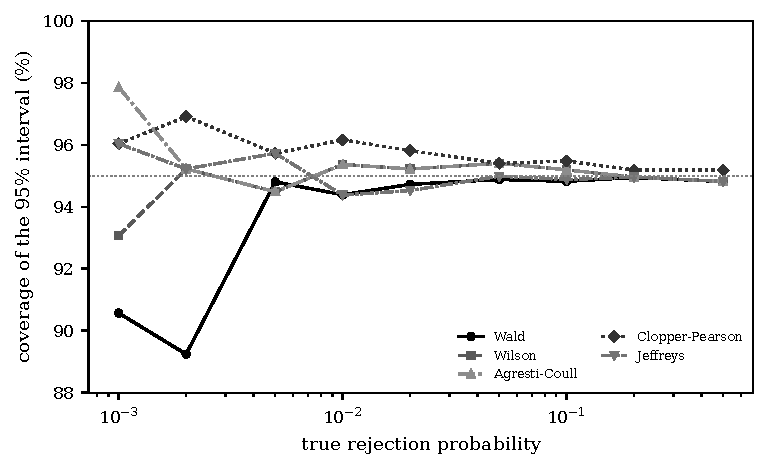
\includegraphics[width=0.85\linewidth]{interval_coverage}
\caption{Exact coverage of five nominal 95\% intervals for a rejection rate measured in 4,000 repetitions, against the true rejection probability on a logarithmic axis: the normal approximation falls well below the nominal coverage at small rates, and the Wilson, Agresti--Coull, Clopper--Pearson and Jeffreys intervals stay near it.}
\label{fig:interval-coverage}
\end{figure}

\subsection{The rule that judges a size}
\label{sec:ab-bound}

The one-sided bound of \eqref{eq:bound}, the screen, and the interval of the definition are compared with the rule that a rate above the level is oversized, on the fifty blocks of every test, grouped by the pooled size of the test (\cref{tab:resolution} and \cref{fig:resolution}).
The group within the level holds conservative tests, whose rate falls away from the level as the cells grow, and tests whose size equals the level, which exceed it in about half of their cells whatever the number of repetitions.
Among the \nWithin{} tests whose pooled size is within the level, the naive rule flags \flWithinNaiveFour\,\% of the cells of 4,000 repetitions, \flWithinNaiveThousand\,\% of the cells of 1,000 and \flWithinNaiveTwentyK\,\% of those of 20,000; the share falls with the repetitions because the conservative tests stop exceeding their level, and it would stay at one half for tests at the level.
The screen flags \flWithinBoundFour\,\% at 4,000 and \flWithinBoundThousand\,\% at 1,000, which is the false flag probability of \cref{prop:false-flag}, and the definition flags \flWithinIntFour\,\% at 4,000 and \flWithinIntThousand\,\% at 1,000, a share below its false flag probability of lagIntFour\,\% for a test at its level, because most of the group is conservative.
Among the \nOver{} tests whose pooled size is above the level, the naive rule flags \flOverNaiveFour\,\% of the cells, the screen \flOverBoundFour\,\% and the definition \flOverIntFour\,\%, and at 20,000 repetitions \flOverNaiveTwentyK\,\%, \flOverBoundTwentyK\,\% and \flOverIntTwentyK\,\%.
The two rules pay for their specificity with sensitivity, the screen more than the definition, and the price is the resolution of \cref{prop:resolution}, not a flaw of the rules: seven of the nine tests above the level exceed it by less than a third of a point.
A reader who needs to see them needs more repetitions, and the naive rule offers no way to know that it has seen them.

\begin{table*}[htbp]
\centering
\footnotesize
\caption{Resolution of a size measurement by the number of repetitions: the excess over the level (percentage points) that the one-sided bound of the screen and the Wilson interval of the definition detect with probability 0.8, and the share of cells (percent) flagged by the naive rule, the screen and the definition among the 10 tests whose pooled size is within the level and among the 9 whose pooled size is above it.}
\label{tab:resolution}
\fitwidth{\begin{tabular}{lrrrrrrrrrr}
\toprule
Repetitions & Screen sees, 5\% & Screen sees, 1\% & Definition sees, 5\% & Definition sees, 1\% & Within: naive & Within: screen & Within: definition & Above: naive & Above: screen & Above: definition \\
\midrule
1,000 & 2.87 & 1.36 & 2.03 & 1.03 & 22.7 & 0.15 & 1.10 & 77.6 & 13.0 & 21.7 \\
2,000 & 2.01 & 0.94 & 1.44 & 0.67 & 19.4 & 0.00 & 0.90 & 82.1 & 13.7 & 27.4 \\
4,000 & 1.39 & 0.66 & 1.00 & 0.47 & 14.0 & 0.00 & 1.60 & 87.8 & 16.4 & 33.3 \\
20,000 & 0.61 & 0.28 & 0.44 & 0.20 & 10.0 & 0.00 & 0.00 & 97.8 & 38.9 & 62.2 \\
200,000 & 0.19 & 0.09 & 0.14 & 0.06 & -- & -- & -- & -- & -- & -- \\
\bottomrule
\end{tabular}}
\end{table*}


\begin{figure}[htbp]
\centering
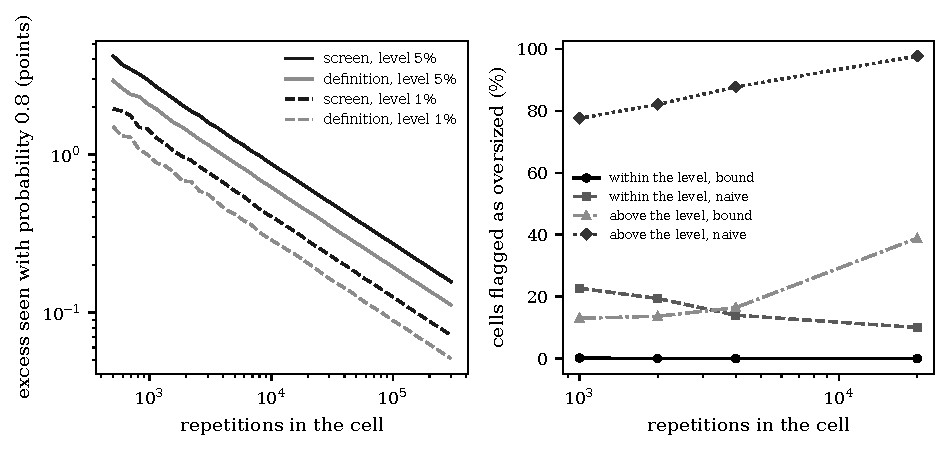
\includegraphics[width=\linewidth]{resolution}
\caption{Left: the excess over the level that the one-sided bound of the screen (black) and the Wilson interval of the definition (grey) detect with probability 0.8 against the number of repetitions of the cell, at the levels 5\% (solid) and 1\% (dashed); right: the share of cells flagged as oversized by the screen and by the naive rule among the tests within the level and among the tests above it.}
\label{fig:resolution}
\end{figure}

\subsection{The exact value beside the rate}
\label{sec:ab-exact}

The exact value does two things that the simulation alone cannot do.
It checks the generator: a generator whose probability of default is 5\,\% too high makes the binomial test reject \agMeanRateFive\,\% of the samples at the 5\,\% level instead of \binExactFive\,\%, which exceeds the bound of \boundFive\,\% and would read as an oversized test, when the defect is in the generator.
The agreement check of \eqref{eq:agree} flags that generator with probability \agFailFivePercent\,\% by exact calculation, and in \agSimFive\,\% of \agBlocks{} simulated blocks (\agSimTen\,\% for a probability of default 10\,\% too high), while it flags the correct generator in \agSimNone\,\% of the blocks, against the \agFailOne\,\% that the calculation gives.
A probability of default 2\,\% too high is flagged with probability \agFailTwoPercent\,\%: the check does not see errors of that size, and the limitations say so.
It also decides what the simulation cannot: the exact size of the Jeffreys test at 1\,\% is \jeffExactOne\,\%, above the level, and one cell of 4,000 repetitions flags an excess of that size with probability \jeffDetect\,\%.

\subsection{The number of repetitions}
\label{sec:ab-repetitions}

The number of repetitions sets the resolution.
\Cref{tab:resolution} gives the excess over the level that the bound sees with probability 0.8: \detFiveThousand{} points at 5\,\% for 1,000 repetitions, \detFiveFour{} for 4,000, \detFiveTwentyK{} for 20,000 and \detFiveTwoHundredK{} for 200,000, and \detOneThousand{}, \detOneFour{}, \detOneTwentyK{} and \detOneTwoHundredK{} points at 1\,\%.
The false flag probability of a test per cell is \flagThousand\,\% at 1,000 repetitions, \flagTest\,\% at 4,000 and \flagTwentyK\,\% at 20,000, so more repetitions buy resolution without costing specificity.
The cost is linear in the repetitions: the 200,000 repetitions per test of the replication, for the 21 tests, took \seedMinutes{} minutes on 24 worker processes.
Four thousand repetitions per size cell is a reasonable default for a first measurement, because it makes the standard error of a rate at 5\,\% about 0.3 points; it is not enough to certify a size, and the replication shows that a result of ``holds'' at 4,000 is a statement of no excess larger than about a point (\detIntFiveFour{} by the definition, \detFiveFour{} by the screen). A user who needs a size known to a tenth of a point must run 200,000 repetitions, and a user who needs only to exclude an excess of three points can run 1,000.

\section{Discussion}
\label{sec:discussion}

\subsection{What a light is worth}
\label{sec:di-lights}

A light is a p-value read against a level, so the rate at which a light is wrongly red is the size of the test, and the rate at which it is rightly red is its power against the defect that is present.
The measurement turns both into numbers a validator can attach to the light.
For most of the \nTests{} tests the size is close to the level in the scenario measured, and a red light from them in the setting of the generator means what it says.
For the tests that assume independent defaults it does not: at an asset correlation of 10\,\% the binomial test, which is exact at independence, is red for a correct PD in \binRhoOneZeroExact\,\% of portfolios of 1,000 obligors and in \binNRhoTenHundredK\,\% of portfolios of 100,000, and the limit of \cref{prop:clustering} is \binLimitRhoTen\,\%.
A larger portfolio makes that test less trustworthy when defaults cluster, which is the reverse of what a practitioner expects from a larger sample.
The advice of the Basel Committee to read these tests as an early warning \citep{bcbswp14} is therefore a statement about their size, and the measurement quantifies it: an early warning that is raised in a fifth to a third of correct portfolios cannot be a decision.
The chi-square test over grades and the Hosmer--Lemeshow test reject a correct model in \chiRhoOneZero\,\% and \hlRhoTwoZero\,\% of the samples at asset correlations of 10\,\% and 20\,\%, and a validator who reads either as a test of calibration is reading a test of the correlation as well.

\subsection{What the tests cannot see}
\label{sec:di-blind}

The measurement finds four tests that are blind to the defect a validator would expect them to see, and each blindness has a cause that the theory identifies.
The default-profile test compares the distribution of defaults over grades, so it sees the shape of the calibration curve and not its level: it rejects \profKThree\,\% of samples when every probability of default is three times too low.
The characteristic stability index of a leaked feature sees the feature's own distribution, which moves little when the leak is the relation between the feature and the outcome, and so it reaches only \leakCsiTwo\,\% at the largest leak while the AUC test sees the same leak in \leakAucZeroFive\,\% at the middle of its ladder.
The concentration test of the European Central Bank cannot reject at all with ten grades at an initial coefficient of variation of 0.6 (\cref{prop:hhi}; with \hhiKMinThree{} grades it can at 0.3), and the chi-square test of homogeneity on the counts, applied to the same samples, rejects \chiCountZeroZeroFive\,\% at 5\,\% of mass moved.
The Vasicek-corrected binomial test pays for protecting against a correlation that the generator does not have, and rejects nothing until the true probability of default is far above the one applied.
Blindness of this kind is not a flaw of a test that is used for what it tests; it is a flaw of a validation report that uses one of these tests as evidence for something else, and the measured power says which.

A second kind of weakness is lack of power at the sample size of the portfolio: with 150 defaulters an AUC drop of two points is caught in \ecbDropZeroTwo\,\% of samples, and the migration z-tests, which control 42 cells with Holm's procedure, miss a migration twice as frequent as its neighbour in about half of the samples with 500 obligors per grade.
The population stability index has the opposite structure: its fixed bands have a false alarm rate that falls with the sample size and a power that depends on the shift only, so the band of 0.10 raises an alarm in \psiHundred\,\% of samples of 100 in which nothing changed (\cref{prop:psi}), and the band of 0.25 raises none for a shift of 0.2 standard deviations in samples of 1,000.

\subsection{What ``holds its size'' means}
\label{sec:di-holds}

The judgement of \cref{def:holds} is a statement of resolution as much as of size, and the paper applies it with one meaning everywhere.
It gives three counts on three bodies of evidence, which \cref{sec:rs-size} reports: \nHoldCellRule{} tests pass the screen on the committed cells of 4,000 repetitions, \nHoldCellDef{} hold their size by the definition on the same cells, and \nHold{} hold it by the definition on the pool of \nRepsPooled{} repetitions, with \nNotHold{} shown above their level.
The first two counts say that the cells of \nNullReps{} repetitions did not see \nMissedByCell{} of the nine tests that the pool shows above their level by the definition (\nMissedByCellRule{} by the screen), with excesses of \smallExcMin{} to \smallExcMax{} points, which no cell of that size can see.
The count that the paper states is the last, and it is a count on the best evidence, not a property that more repetitions could not change: a test that holds its size on 200,000 repetitions may be shown above its level by 2,000,000, and the nine are the tests shown above it so far.
Whether such an excess matters is a question for the user of the test, not for the measurement: a size of \pooledPsi\,\% against a level of 5\,\% changes few decisions, and a size of \pooledNorm\,\% changes many.
The measurement offers a way to state the question: the size with its interval, the resolution of the cell, and the group in which the pooled replication places the test.
It does not offer a threshold, and none is implied. The distinction also tells a validator what to ask of an engine: not that every test has a size equal to its level, which only some of the 21 tests of the battery have to the resolution of 200,000 repetitions, but that the departures that matter for decisions, the ones of several points that correlated defaults and wrong reference values produce, are measured and documented.

\subsection{What the measurement changed in the engine}
\label{sec:di-engine}

Several defaults of the engine that is measured were set by measurements of this kind.
The Hosmer--Lemeshow test uses as many degrees of freedom as groups for probabilities that were set before the outcomes, since the two fewer degrees of freedom of the original statistic over-reject by the \hlFitted\,\% of \cref{sec:rs-settings} on a validation sample.
The comparison of the AUC with its development value has an extension that adds the variance of the development estimate, which brings the size from \aucDevOne\,\% to \aucDevOneExt\,\% in the design in which the two samples are of equal size.
The migration z-tests report a Holm-adjusted family-wise p-value, which the measurement shows to be conservative for one planted cell, and the concentration statistic is documented as bounded.
A measurement of size and power is thus a development tool for a validation engine, not only a report on it: the first two of these defaults were choices that a reader of the p-value could not have checked, and the measurement checked them.

\subsection{Reading the extension}
\label{sec:di-extension}

The \nExtTests{} tests outside the credit families are measured at one alternative each and at the null of one study, so their results are less informative than those of the credit families, and \nExtHold{} of them hold their size on a single cell of \nNullReps{} repetitions.
\nExtNotHold{} do not (\cref{sec:extension}), and two of them, the independence and the conditional-coverage tests of Christoffersen, are the tests that the back-testing literature relies on for the clustering of exceedances \citep{christoffersen1998}, and the conditional-coverage test rejects \chrCcFive\,\% of correct models at 5\,\% in series of 1,500 days at a 5\,\% quantile, so that a back-test of 1,500 days read through it flags a correct model in about one case in fifteen; the independence test rejects \chrIndFive\,\% at 5\,\%, within the bound of the screen, and \chrIndOne\,\% at 1\,\%, above it.
The power of the dynamic quantile test of \citet{engle2004} at 250 days and a 1\,\% quantile is \extPowMin\,\%, which says that a series of that length cannot reject a mis-specified VaR model by this test; this is a statement about the test at the stated alternative and not about the risk model. The extension also shows how conservative tests hide in a battery: \nExtCons{} of the 25 studies reject less often than their level, which costs power and not credibility, and a validator who reads a green light from one of them has seen less than the light suggests.

\section{Limitations}
\label{sec:limitations}

\subsection{Internal validity}
\label{sec:li-internal}

The rates are estimates, and each carries its Monte Carlo error; the conclusions that follow from them are limited by it.
A cell of \nNullReps{} repetitions resolves an excess over the level of about \detFiveFour{} points at 5\,\% and \detOneFour{} points at 1\,\%, so the statement that a test holds its size is a statement about excesses larger than that, and the replication shows that \nVerdictDisagree{} of the \nTests{} tests are judged differently by the pool of \nRepsPooled{} repetitions.
A power point of \nPowerReps{} repetitions has a standard error of up to 1.1 points, and the interval of $\hat\sev_{0.8}$ ignores the dependence between neighbouring points.
The agreement check of \eqref{eq:agree} is run on the three count tests and the traffic-lights test only, and it does not see an error of 2\,\% in a probability of default, which it flags with probability \agFailTwoPercent\,\%; a generator error smaller than that would pass.
The exact probabilities exist for four tests of the 21, so for the other 17 the generator is checked by the reruns of published studies, which cover three studies and a fraction of the tests, and by the exact values of the tests that share a generator with them.
The judgement of a battery of 21 tests at two levels is not corrected for multiplicity: if the tests were independent and correct, about \flagFamily\,\% of batteries would flag at least one, and at most \flagUnion\,\% in any case.
The 5\,\% and 1\,\% levels are measured on the same samples, so their rates are not independent.

\subsection{External validity}
\label{sec:li-external}

Every generator is a design choice, and a size measured on one is a property of the test in that scenario.
The size of a count test depends on the number of obligors and on the probability of default: the exact size of the Jeffreys test at 1\,\% is \jeffExactOne\,\% for 1,000 obligors at 1\,\%, and it moves with both because the count is discrete, so another portfolio would give another size, sometimes below the level.
The null generators use independent years, a single systematic factor and normal scores; a portfolio with serial correlation of the systematic factor, several factors, heavy tails or missing values is not represented.
The severity ladders were set from pilot runs so that the power of the targeted tests runs from their size towards one in the sample size of the family, and they are in the units of the generator: a true probability of default that is a multiple of the one applied, an AUC drop, a mean shift in standard deviations of a normal base.
Power against such a ladder is not the probability that a test detects a real problem of a real bank, and the values of $\hat\sev_{0.8}$ compare tests on the same panel and not tests across panels.
The extension to the 21 tests outside the credit families has one alternative per test, no ladder, and a size at the null of one study, so it gives two points per study and no curve.
No real portfolio, real model or real bank enters the measurement; the claim is about the tests, not about any institution.

\subsection{Construct validity}
\label{sec:li-construct}

The measurement counts a rejection when the p-value is below the level, which is the rule of the lights of the engine at the two levels it uses.
A validation report reads several tests together, applies tolerances and judgement, and acts on the pattern; the rejection rate of one test does not give the rate at which a report reaches a wrong conclusion, which would need a model of how reports combine tests.
Four of the 21 tests have no power in the measurement because no defect of the rating process was planted for them, and nothing here says how they perform against a defect.
A threshold, a pass mark or a regulatory limit is not implied by any size or power in the text: the sizes and powers are descriptions of what each test does on the generator it was measured on, and the question of what error rate is acceptable belongs to the user of the test.
The generators and the tests were written by the same programme, so the measurement checks the engine against the truth of its own generators, and independent implementations of the tests, which the published reruns and the recomputation of the binomial rejection probability partly provide, would strengthen it.
Finally, the measurement is of one release of the engine, 1.1.0, and a later release that changes a test changes its size and its power; the repository's scripts rerun every number.

\section{Reproducibility}
\label{sec:reproducibility}

Every number of the text comes from the committed documents under \texttt{data/derived/C22} or from the compact results of the three experiments under \texttt{experiments/results}, through the scripts of the manuscript folder; no number is typed.
The scripts run with the Python environment of the engine (\texttt{riskvalidation} 1.1.0 with its market, machine-learning and stress extras, NumPy \citep{harris2020} and SciPy \citep{virtanen2020}) and read no data outside the repository; a random stream is a function of its seed and the index of the repetition, so a rerun on another machine returns the same counts.

The commands, run from the manuscript folder of the repository, are the following.
\begin{verbatim}
python experiments/exp_reproduce.py
python experiments/exp_seed_replication.py
python experiments/exp_instrument.py
python make_numbers.py
python make_tables.py
python make_figures.py
python fetch_references.py
\end{verbatim}
The first reruns the 21 committed null cells with their seeds and takes \reproSeconds{} seconds on six worker processes; the second measures each test in 50 further blocks of 4,000 repetitions and takes \seedMinutes{} minutes; the third computes the exact probabilities of the instrument and 600 simulated blocks and takes \instrMinutes{} minutes in one process.
Their outputs are the JSON files of \texttt{experiments/results}, each under 250 kilobytes.
The next three scripts regenerate the numbers file, the tables and the vector figures from the documents and the results, and the last writes the bibliography from the publishers' records of the works that the text cites.
The document is built with \texttt{pdflatex}, \texttt{bibtex} and two further passes of \texttt{pdflatex} from the manuscript folder.

The repository, its releases and its committed artifacts are named in the header of the first page, and the cases of the repository record, for every committed document, the seed of the case, the version of the engine and the generators that were drawn.
The practice follows the recommendations on the computational reproducibility of research \citep{sandve2013}: every result has a script, every random number has a seed, and the version of every program is recorded.

\section{Conclusions}
\label{sec:conclusions}

The size and the power of validation tests can be measured, with their error, on generators whose truth is known, and the measurement changes what the lights of a validation report are taken to mean.
Of the \nTests{} tests of the credit families, \nHold{} hold their size at 5\,\% and 1\,\% in cells of \nNullReps{} repetitions, and \nNotHold{} do not: the Jeffreys test of the default probability has an exact size of \jeffExactOne\,\% at the 1\,\% level, and the normal test over five years rejects \normFive\,\% of correct models at 5\,\%.
The resolution of a cell is about \detFiveFour{} points, \nBlocks{} independent blocks show that \nSmallOver{} further tests exceed their level by \smallExcMin{} to \smallExcMax{} points, and the judgement of a single cell differs from that of the pool for \nVerdictDisagree{} tests; a statement that a test holds its size is a statement with a resolution.
The largest departures come from assumptions that fail in real portfolios, and they are explained by short derivations: defaults that are correlated give the binomial test a size of \binRhoOneZeroExact\,\% at an asset correlation of 10\,\% in a portfolio of 1,000 and a limit of \binLimitRhoTen\,\% for large portfolios, a degrees-of-freedom convention and a reference value that is an estimate move a size to \hlFitted\,\% and \aucDevOne\,\%, a fixed band of the stability index alarms in \psiHundred\,\% of samples of 100 in which nothing changed, and a bounded statistic gives the concentration test no power at all with ten grades.
On power, \nReach{} of the \nPowerTests{} tests reach 80\,\% on the ladder of the defect planted for them, and the Vasicek-corrected binomial test, the default-profile test, the characteristic stability index and the concentration test do not.
The instrument is sound where it can be checked: all \nAgree{} exact comparisons agree, the three published simulation studies that can be rerun are rerun with \wpAgree{} of \wpTotal{} and \ynAgree{} of \ynTotal{} cells reproduced, and all \nReproTotal{} committed cells reproduce exactly from their seeds.
Three of the eight predictions of the design are refuted, those on the size of every test, on the stability of a single cell's judgement and on the reach of every power curve, and they are reported as such.

The measurement has limits that the generators and ladders impose: it describes the tests on the scenarios it draws, it does not describe a bank, and it implies no threshold.
The next steps are to plant defects of the transition process, so that the four transition tests have a power, to extend the generators to serial correlation of the systematic factor and to several factors, to run the extension tests along ladders, and to repeat the measurement on each new release of the engine, since a test that changes changes its size and its power.


\bibliographystyle{plainnat}
\bibliography{references}

\end{document}
